\chapter{Referencial Teórico}

Neste capítulo serão abordados os tópicos considerados mais relevantes para atingir o embasamento teórico necessário para a realização deste trabalho.

\section{Redes Sociais}

Quando se pensa em rede, surge a ideia de um conjunto de nós interligados entre si, como uma teia que ocupa um determinado espaço em um ambiente. Os nós ou pontos estão ligados em pares e podem representar várias situações em áreas de interesse em comum \cite{Newman:2010}.

Para Sodré \cite{Sodre:2002}, rede é onde as conexões e as interseções tomam o lugar do que seria antes apenas linearidade. Essas conexões e interações ocorrem pelo contato direto, face a face, e pelo contato indireto, utilizando-se um veículo mediador, como o telefone.

As pessoas estão inseridas na sociedade por meio das relações que desenvolvem durante toda sua vida, primeiro no âmbito familiar, em seguida na escola, na comunidade em que vivem e no trabalho; enfim, as relações que as pessoas desenvolvem e mantêm é que fortalecem a esfera social. A própria natureza humana nos liga a outras pessoas e estrutura a sociedade em rede \cite{Tomae:Alcara:Chiara:2005}.

Os tipos de relações também podem ser de movimentação entre lugares, como migração, mobilidade física ou social, conexão física, como uma estrada, um rio ou uma ponte que conecta dois lugares, de relações de autoridade ou relação biológica, como descendência, por exemplo \cite{Wasserman:1994}.

Com base em seu dinamismo, as redes, dentro do ambiente organizacional, funcionam como espaços para o compartilhamento de informação e do conhecimento. Espaços que podem ser tanto presenciais quanto virtuais, em que pessoas com os mesmos objetivos trocam experiências, criando bases e gerando informações relevantes para o setor em que atuam \cite{Tomae:Alcara:Chiara:2005}.

\begin{quote}
	``[...] na era da informação – na qual vivemos – as
	funções e processos sociais organizam-se cada vez
	mais em torno de redes. Quer se trate das grandes
	empresas, do mercado financeiro, dos meios de
	comunicação ou das novas ONGs globais,
	constatamos que a organização em rede tornou-se
	um fenômeno social importante e uma fonte crítica
	de poder.'' \cite{Capra:2002}
\end{quote}

O contexto em que estamos inseridos desencadeia uma série de mudanças na rotina dos indivíduos, e uma delas evidencia as redes como ponto de convergência da informação e do conhecimento \cite{Tomae:Alcara:Chiara:2005}.

O conhecimento que a rede possui repercute sobre o meio que esta se encontra, pois Wellman \cite{Wellman:1996} verifica, na rede, sua identidade singular em determinada situação, isto é, a representação e a interpretação das relações em rede estão fortemente ligadas à realidade que a cerca; a rede é influenciada pelo seu contexto e esse por ela. Portanto, para \cite{Marteleto:2001}, os efeitos das redes podem ser percebidos fora de seu espaço, nas interações com o estado, na sociedade ou outras instituições representativas.

A interação constante ocasiona mudanças estruturais e, em relação às interações em que a troca é a informação, a mudança estrutural que pode ser percebida é a do conhecimento. Quanto mais informação trocamos com o ambiente que nos cerca, com os atores da nossa rede, maior será nossa bagagem de conhecimento, maior será nosso estoque de informação, e é nesse conjunto de significados que inserimos as redes sociais \cite{Tomae:Alcara:Chiara:2005}.

Milgram, em sua tese \cite{Milgram:1967}, defende que qualquer pessoa está distante de qualquer outra pessoa do mundo, a no máximo seis graus de separação. Essa tese ficou conhecida como ``mundo pequeno'' e ``teoria dos seis degraus''. Sua pesquisa demonstra que a rede social constitui importante recurso profissional e pessoal. Estar em contato com pessoas que conheçam uma pessoa-alvo, em razão de um interesse específico, já é um passo além para a conquista de um objetivo.

\section{Teoria dos Grafos}

O desenvolvimento da análise de redes sociais tem como fundamento a teoria dos grafos, a seguir serão apresentados os principais conceitos sobre grafos.

\subsection{História}

O primeiro livro sobre a teoria dos grafos foi publicado por König (1936). Isso levou ao desenvolvimento de uma forte escola de teóricos em grafos na Hungria que incluíram P. Erdős e T. Gallai. Também na década de trinta, H. Whitney publicou uma série de artigos influentes \cite{Bondy:2007}.

De acordo com Ore \cite{Ore:1963}, Leonhard Euler\footnote{Grande matemático e físico suíço, 1707-1783, fez importantes descobertas em campos variados como Cálculo e Grafos.} teria sido um dos matemáticos mais importantes quando se refere a teoria dos grafos. Contam que o povo da cidade de Königsberg \footnote{atualmente Caliningrado.}, localizado na Prússia e cortada pelo Rio Pregel, com sete pontes ligando duas ilhas e as margens opostas do rio, como pode ser visto na Figura \ref{Konigsberg}, propôs ao então famoso matemático Leonard Euler o seguinte problema:

	“Será possível fazer um passeio pela cidade, começando e
	terminando no mesmo lugar, cruzando cada ponte exatamente uma vez?”

\begin{figure}[!h]
	\centering
	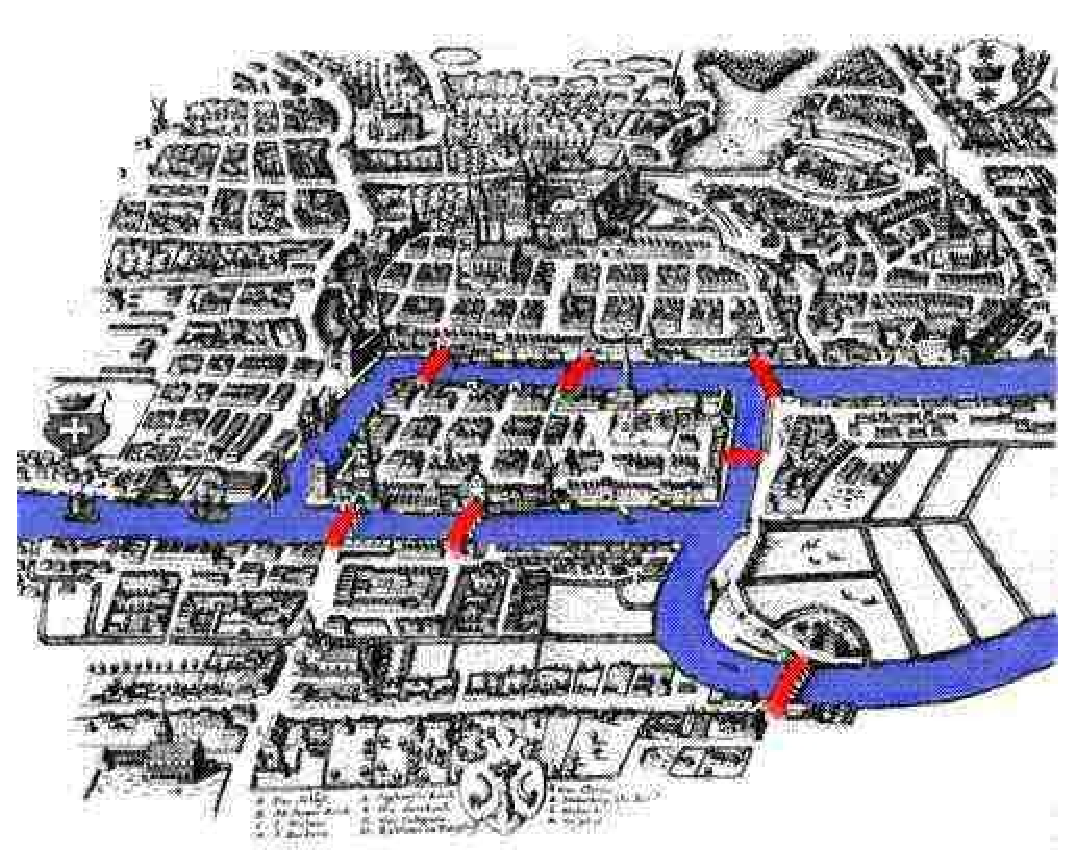
\includegraphics[scale=0.35]{figuras/capitulo2/Konigsberg.eps}
	\caption{Pontes de Königsberg}
	\label{Konigsberg}
\end{figure}

Não se sabe se Euler teria resolvido usando a representação de grafos que adotamos hoje. A modelagem do problema por grafo passa pela representação onde cada porção de terra  é representada por um ponto e as pontes estariam representadas por linhas \cite{Ore:1963}, apresentado na Figura \ref{sete_pontes}.

\begin{figure}[!h]
	\centering
	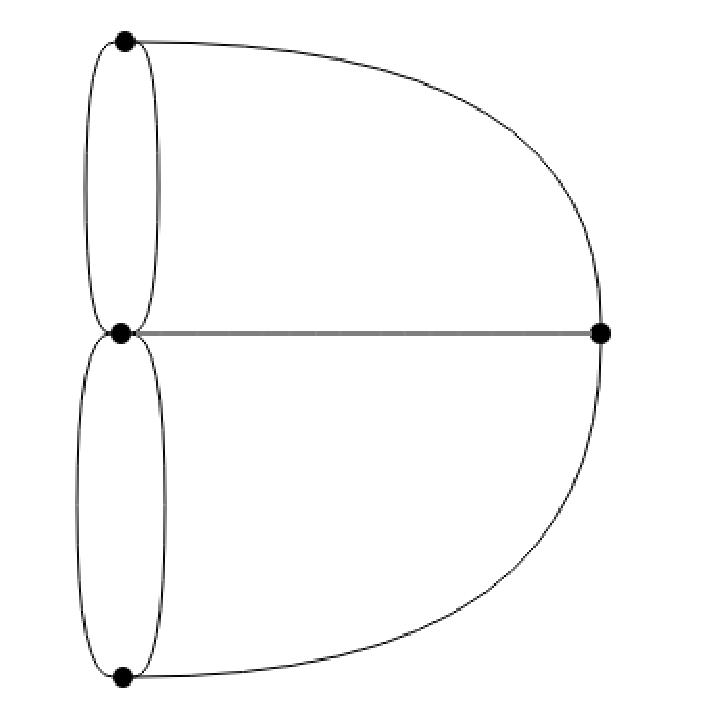
\includegraphics[scale=0.25]{figuras/capitulo2/sete_pontes.eps}
	\caption{Problema das sete pontes}
	\label{sete_pontes}
\end{figure}

Analisando, então, este grafo, Euler resolveu a questão provando que uma caminhada assim é possível se, e somente se, o grafo for conexo e todos os seus vértices tiverem grau par, termos estes que serão tratados mais à frente \cite{Malta:2008}.

Assim, Euler mostrou que, uma vez que o grafo de Königsberg tem vértices de grau ímpar, a resposta ao problema era que tal caminhada era impossível. Desde então, todo grafo conexo, cujos vértices possui grau par, é chamado de grafo euleriano, e um caminho fechado em um grafo que passe por cada aresta deste exatamente uma vez é chamado de circuito (ou ciclo) euleriano \cite{Malta:2008}.

Graças à resolução dada por Euler, mais tarde muitos outros problemas importantes, para o desenvolvimento da Matemática Aplicada, foram possíveis de serem modelados. Um desses modelos são as relações de amizade, de hierarquia, de trabalho. Netto \cite{Netto:2012}, aponta grafos como um auxílio para o estudo de problemas envolvendo inter-relacionamento de elementos (em química orgânica, eletricidade, organização, transporte, psicossociologia). Na verdade, grafos modelam diversas situações e muitas delas não quantificáveis.

Conforme Ore \cite{Ore:1963}, no século seguinte, o matemático irlandês William Hamilton, em 1859, inventou um jogo chamado ``\textit{The Icosian Game}'', com um peculiar enigma envolvendo um dodecaedro, em que cada um dos 20 vértices foram nomeados com nomes de cidades importantes. O objetivo do jogo era, utilizando as 30 arestas do dodecaedro, passar por cada uma das cidades apenas uma vez, começando e terminando na mesma cidade. Um exemplo do grafo pode ser visualizado na Figura \ref{grafo_hamiltoniano}.

\begin{figure}[!h]
	\centering
	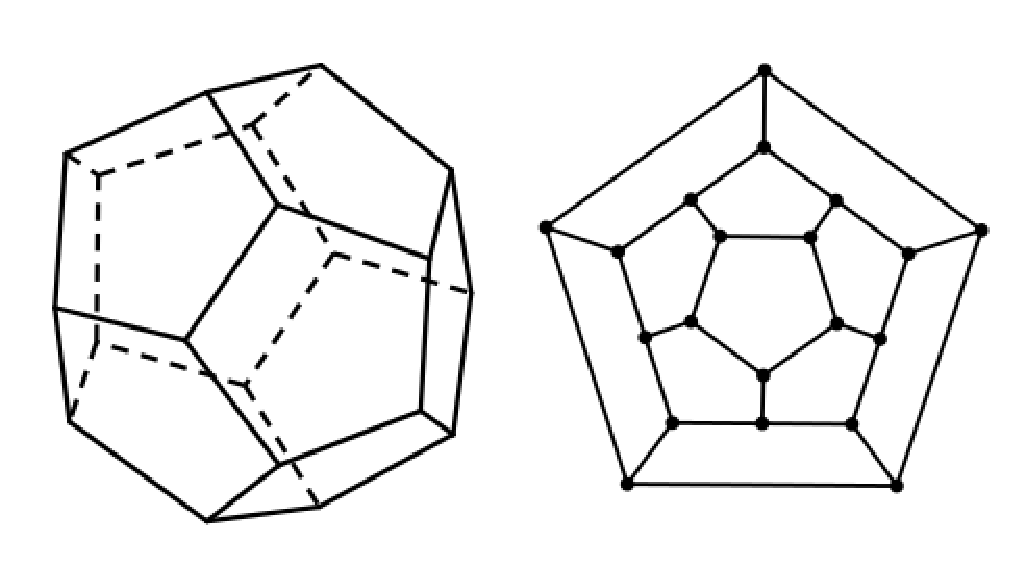
\includegraphics[scale=0.3]{figuras/capitulo2/grafo_hamiltoniano.eps}
	\caption{Grafo hamiltoniano}
	\label{grafo_hamiltoniano}
\end{figure}

Apesar da simples formulação, o problema admite muitos caminhos como resposta. No problema de Hamilton, temos uma diferença significativa em relação ao problema de Euler. Encontrar um caminho euleriano significa encontrar um caminho que passe por todas as arestas do grafo uma única vez, podendo ser aberto ou fechado. Nos caminhos hamiltonianos, cada vértice é visitado uma única vez. O problema fica muito mais complexo com tal condição \cite{Costa:2011}.

\subsection{Definições}

\textbf{Definição 1}: Um grafo \textit{G} é um par ordenado (\textit{V}(\textit{G}), \textit{E}(\textit{G})). Que consiste de um conjunto \textit{V}(\textit{G}) de vértices, um conjunto \textit{E}(\textit{G}), disjunto de \textit{V}(\textit{G}), de arestas, e uma função de incidência $\psi_G$ que associa a cada aresta de \textit{G} um par não ordenado de (não necessariamente distintas) vértices de \textit{G} \cite{Bondy:2007}.

\textbf{Definição 2}: Um grafo é um par \textit{G} = (\textit{V}, \textit{E}) de conjuntos de tal modo que \textit{E}$\subseteq$[\textit{V}$_2$]; Assim, os elementos de \textit{E} são subconjuntos de pares ordenados de elementos de \textit{V}. Para evitar ambiguidades de notação, deve-se sempre assumir implicitamente que \textit{V}$\cap$\textit{E}=$\oslash$. Os elementos de \textit{V} são os vértices (ou nós ou pontos) do grafo \textit{G}, os elementos de \textit{E} são arestas (ou linhas) \cite{Diestel:1997}.

Grafos são assim chamados porque eles podem ser representados graficamente, e é esta representação gráfica que nos ajuda a entender muitas de suas propriedades. Cada vértice é indicado por um ponto, e de cada aresta por uma linha que une os pontos que representam as suas extremidades \cite{Bondy:2007}. Um exemplo pode ser observado na Figura \ref{exemplo_grafo}.

\begin{figure}[!h]
	\centering
	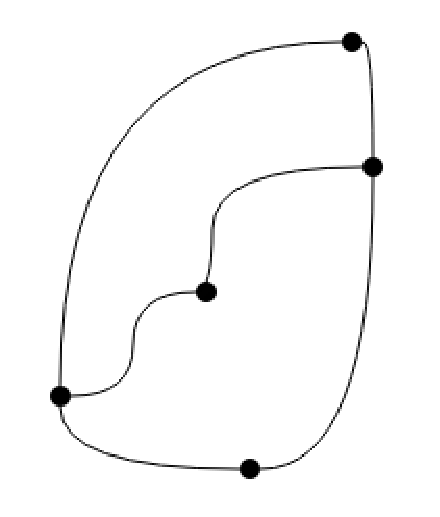
\includegraphics[scale=0.3]{figuras/capitulo2/exemplo_grafo.eps}
	\caption{Exemplo de grafo}
	\label{exemplo_grafo}
\end{figure}

A maioria das definições e conceitos na teoria dos grafos são sugeridas por esta representação gráfica. As extremidades de uma aresta são referidas como sendo incidente com a aresta, e vice-versa. Dois vértices que são incidentes com uma aresta em comum são chamados de adjacentes, e dois vértices adjacentes distintos são chamados de vizinhos \cite{Costa:2011}.

Uma aresta com extremidades idênticas é chamada um \textit{loop}, e uma aresta com extremidades distintas é um \textit{link}. Dois ou mais \textit{links} com o mesmo par de extremidades são referidos como sendo arestas paralelas \cite{Bondy:2007}. Na Figura \ref{loop_paralela}, é possível observar a aresta ``a'' como uma aresta do tipo \textit{loop}, e as arestas ``b'' e ``e'' como arestas do tipo \textit{link} e as aresta ``c'' e ``d'' como sendo arestas paralelas.

\begin{figure}[!h]
	\centering
	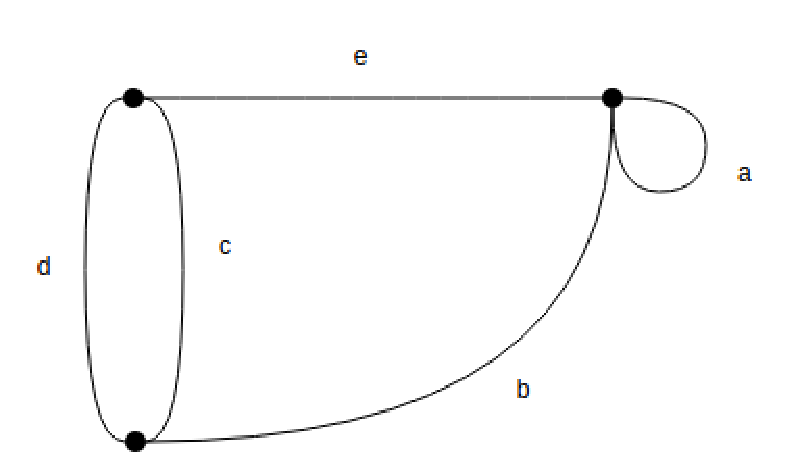
\includegraphics[scale=0.4]{figuras/capitulo2/loop_paralela.eps}
	\caption{Exemplo de loop e arestas paralelas}
	\label{loop_paralela}
\end{figure}

Um grafo é finito se tanto o seu conjunto de vértices, quanto o seu conjunto de arestas são finitos. Um grafo sem vértices (e, portanto, sem arestas) é o grafo nulo. Qualquer grafo apenas com um vértice é referido como trivial. Todos os outros grafos são não-triviais \cite{Costa:2011}.

Um grafo é simples se não tem \textit{loops} ou arestas paralelas \cite{Diestel:1997}, como exemplificado na Figura \ref{grafo_simples}.

\begin{figure}[!h]
	\centering
	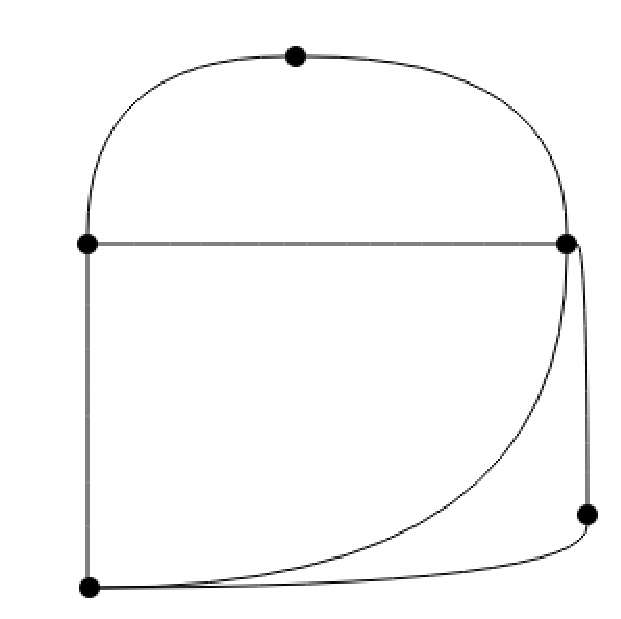
\includegraphics[scale=0.2]{figuras/capitulo2/grafo_simples.eps}
	\caption{Exemplo de grafo simples}
	\label{grafo_simples}
\end{figure}

Certos tipos de grafos podem desempenhar papéis proeminentes na teoria dos grafos. Um grafo conexo é um grafo simples no qual quaisquer dois vértices são ligados por um caminho. Um grafo é vazio quando não há dois vértices adjacentes (isto é, o conjunto de arestas é vazio). Um grafo é bipartido se o seu conjunto de vértices pode ser particionado em dois subconjuntos \textit{X} e \textit{Y} para que cada aresta tem um fim em \textit{X} e um fim em \textit{Y}; uma tal partição (\textit{X}, \textit{Y}) é chamada uma bipartição do grafo, e \textit{X} e \textit{Y} suas partes. Pode-se denotar um grafo bipartido \textit{G} com bipartição (\textit{X}, \textit{Y}) por \textit{G}[\textit{X}, \textit{Y}]. Se \textit{G}[\textit{X}, \textit{Y}] é simples e todos os vértices de \textit{X} estão associados a cada vértice em \textit{Y}, então \textit{G} é chamado de um grafo bipartido completo. Uma estrela é um grafo bipartido completo \textit{G}[\textit{X}, \textit{Y}] com |\textit{X}| = 1 ou |\textit{Y}| = 1 \cite{Diestel:1997}.  A Figura \ref{tipos_grafos} ilustra estes tipos de grafos, sendo o grafo ``A'' é um grafo conexo, o grafo ``B'' é um grafo vazio e o grafo ``C'' é um grafo bipartido completo.

\begin{figure}[!h]
	\centering
	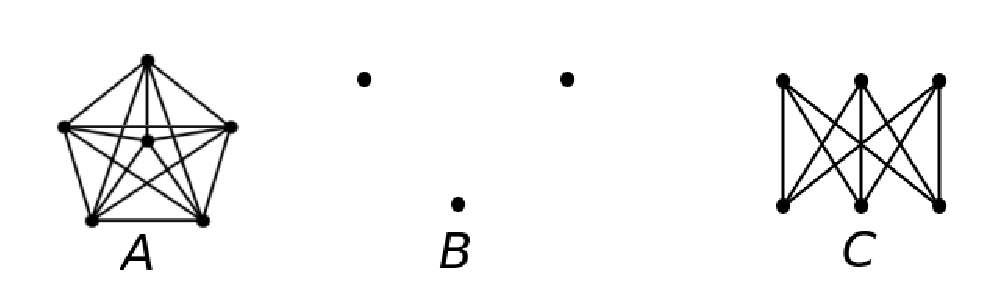
\includegraphics[scale=0.4]{figuras/capitulo2/tipos_grafos.eps}
	\caption{Tipos de grafos}
	\label{tipos_grafos}
\end{figure}

Um caminho é um grafo simples cujos vértices podem ser dispostos em uma sequência linear. De tal forma que dois vértices são adjacentes se forem consecutivos na sequência, e não adjacentes caso não forem consecutivos \cite{Bondy:2007}. Dessa forma, diz-se que um vértice é alcançável a partir de outro, se houver um caminho levando o primeiro vértice ao último \cite{Costa:2011}. A Figura \ref{caminho} apresenta um caminho (arestas em vermelho) do vértice ``a'' até o vértice ``e''.

\begin{figure}[!h]
	\centering
	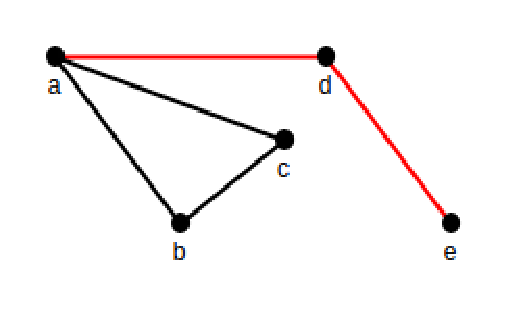
\includegraphics[scale=0.5]{figuras/capitulo2/caminho.eps}
	\caption{Caminho}
	\label{caminho}
\end{figure}

Do mesmo modo, um ciclo é um grafo simples cujos vértices podem ser dispostos em uma sequência cíclica de tal maneira que dois vértices são adjacentes se forem consecutivos na sequência. O comprimento de um caminho ou de um ciclo é o número de suas arestas \cite{Costa:2011}. É possível observar na Figura \ref{ciclos} alguns exemplos de grafos com ciclo.

\begin{figure}[!h]
	\centering
	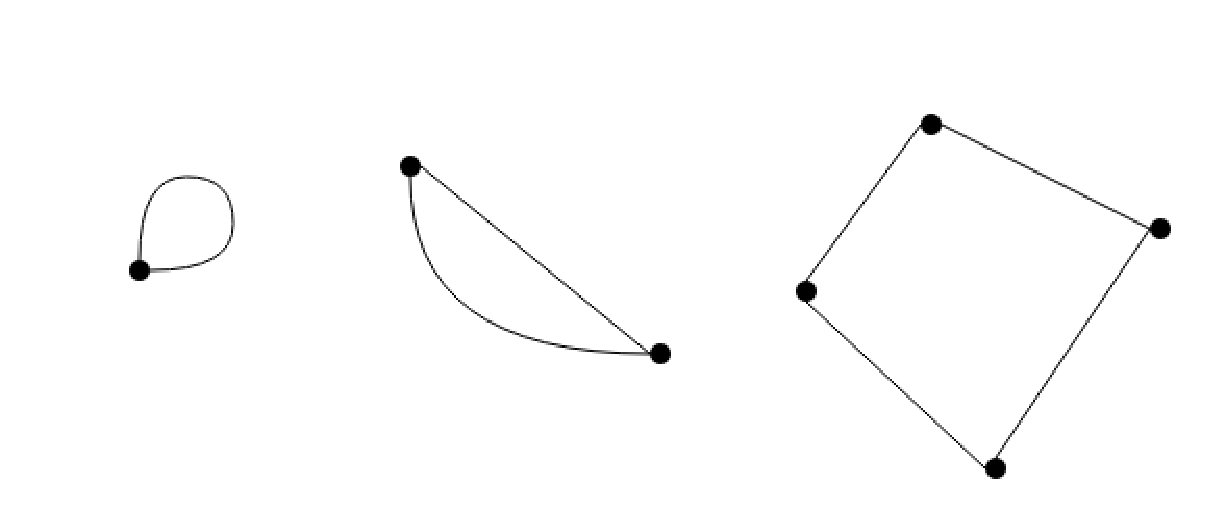
\includegraphics[scale=0.3]{figuras/capitulo2/ciclos.eps}
	\caption{Exemplo de grafos com ciclos}
	\label{ciclos}
\end{figure}

Um grafo é conectado se, para cada partição de seus vértices definido em dois conjuntos \textit{X} e \textit{Y} não vazios, existe uma aresta com uma extremidade em \textit{X} e uma extremidade em \textit{Y}; caso contrário, o grafo é desconectado. Em outras palavras, um grafo é desconectado se o conjunto de vértices pode ser particionado em dois subconjuntos não vazios \textit{X} e \textit{Y} e que nenhuma aresta tem uma extremidade em \textit{X} e a outra extremidade em \textit{Y}. É instrutivo comparar esta definição com a de um grafo bipartido. Os exemplos de grafos conectados e desconectados são apresentados na Figura \ref{desconectados}, onde o grafo ``X'' e o grafo ``Y'' são dois grafos distintos conectados. Porém se fossem trados como um único grafo, este seria um grafo desconectado \cite{Bondy:2007}.

\begin{figure}[!h]
	\centering
	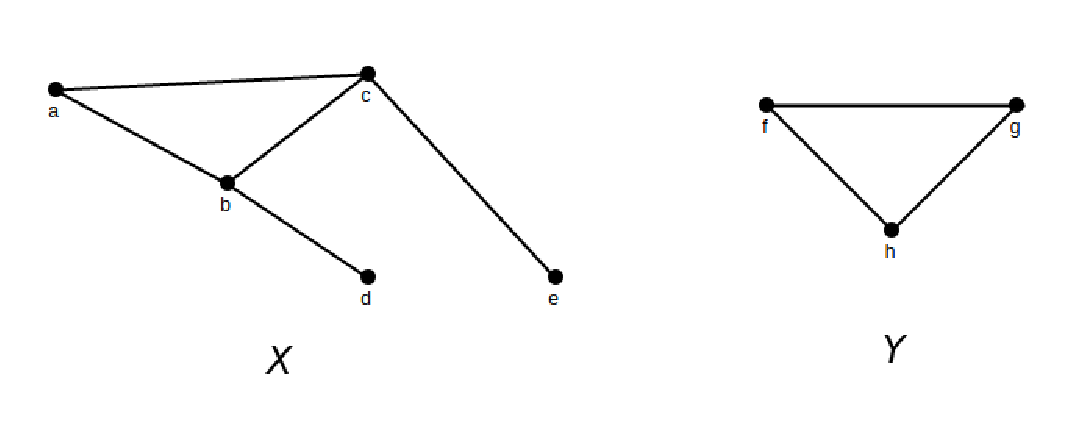
\includegraphics[scale=0.45]{figuras/capitulo2/desconectados.eps}
	\caption{Exemplo de grafos conectados e desconectados}
	\label{desconectados}
\end{figure}

O grau de um vértice \textit{v} em um grafo \textit{G}, designado por \textit{d$_G$}(\textit{v}), é o número de arestas de \textit{G} que incidem em \textit{v}; para cada \textit{loop} é contado duas arestas. Em particular, se \textit{G} é um grafo simples, \textit{d$_G$}(\textit{v}) é o número de vizinhos de \textit{v} em \textit{G}. Um vértice de grau zero é chamado um vértice isolado. Denominamos por $\delta$(\textit{G}) e $\Delta$(\textit{G}) mínimo e máximo graus dos vértices de \textit{G}, e por \textit{d}(\textit{G}), o seu grau médio, $\frac{1}{n}\sum_{\textit{v}\in\textit{V}} \textit{d}(\textit{v})$ \cite{Diestel:1997}.	

\subsection{Representação de Grafos}

Embora desenhos são um meio conveniente de especificação de grafos, eles claramente não são adequados para armazenar grafos em computadores, ou para a aplicação de métodos matemáticos para estudar suas propriedades. Para estes fins, são consideradas duas matrizes associadas com um grafo; uma matriz de incidência e uma matriz de adjacência \cite{Bondy:2007}.

Seja \textit{G} um grafo, com conjunto de vértices \textit{V} e conjunto de arestas \textit{E}. A matriz de incidência de \textit{G} é a matriz $M_G:= (m_{ve})$, com dimensões \textit{n$\times$m}, onde $m_{ve}$ é o número de vezes (0, 1, ou 2) que o vértice \textit{v} e aresta \textit{e} estão conectados \cite{Bondy:2007}.

A matriz de adjacência de \textit{G} é a matriz $A_G := (a_{uv})$, com dimensões \textit{n$\times$n}, em que $a_{uv}$ é o número de arestas que unem os vértices \textit{u} e \textit{v}, onde cada \textit{loop} conta como duas arestas. É possível verificar que a quantidade de memória necessária para essa representação é $\Theta(|\textit{V}|^2)$ \cite{Bondy:2007}. A Figura \ref{matriz} ilustra um grafo \textit{G} representado na matriz de incidência \textit{M} e na matriz de adjacência \textit{A}.

\newpage

\begin{figure}[!h]
	\centering
	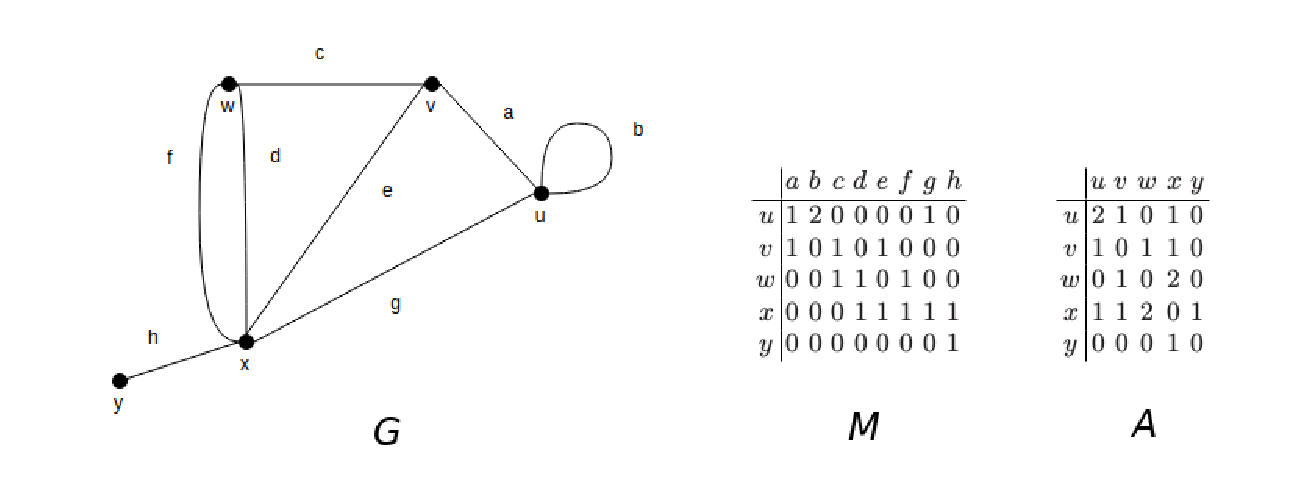
\includegraphics[scale=0.6]{figuras/capitulo2/matriz.eps}
	\caption{Representação em matriz}
	\label{matriz}
\end{figure}

Pela maioria dos grafos possuírem um número bem maior de arestas do que os vértices, a matriz de adjacência de um grafo geralmente é menor do que a sua matriz de incidência e, assim, necessita de menos espaço de armazenamento. Ao lidar com grafos simples, uma representação ainda mais otimizada é possível. Para cada vértice \textit{v}, os vizinhos de \textit{v} são armazenados em uma lista. A lista (\textit{N}(\textit{v}): \textit{v $\in$ V}) é chamada de lista de adjacência do grafo, onde \textit{N}(\textit{v}) representa os vizinhos do vértice \textit{v}. Um exemplo pode ser observado na Figura \ref{lista_adjacencia}. A quantidade de memória necessária para uma lista de adjacências é $\Theta(|\textit{V}| + |\textit{E}|)$. Grafos simples são normalmente armazenados em computadores como listas de adjacência \cite{Costa:2011}.

\begin{figure}[!h]
	\centering
	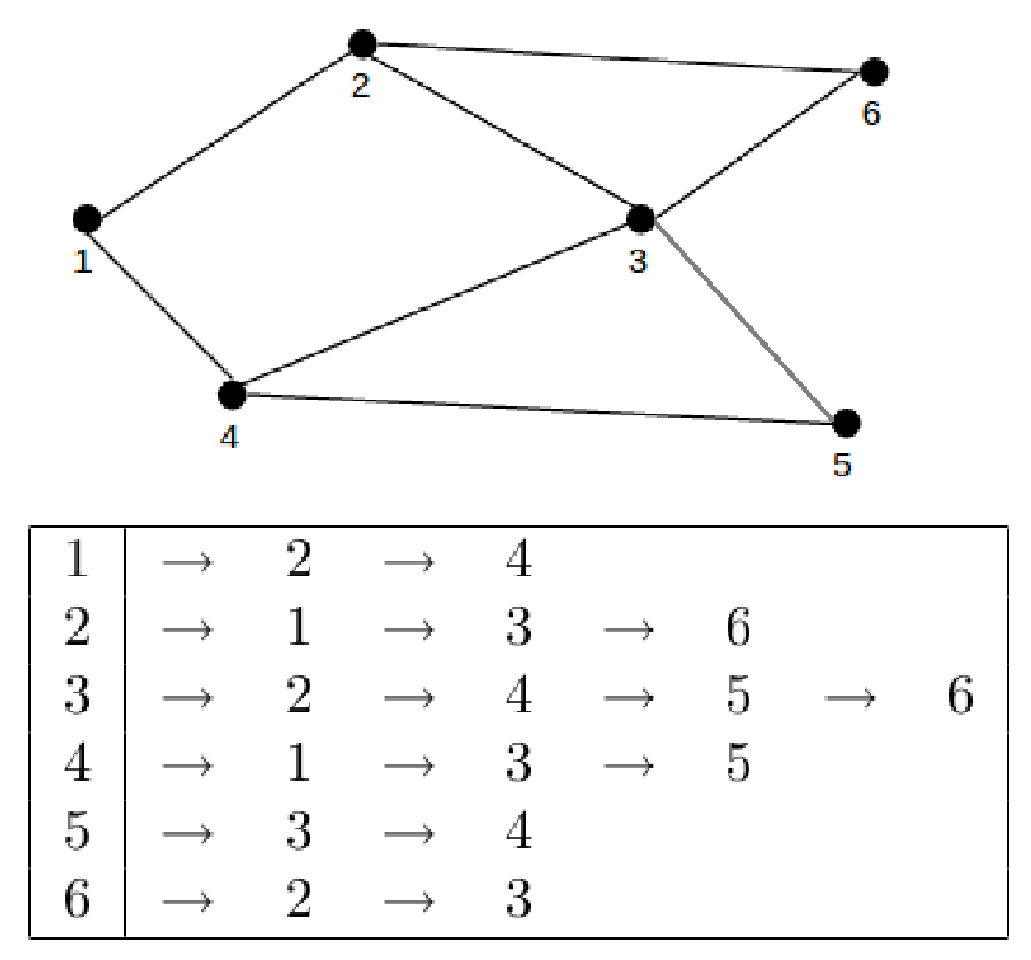
\includegraphics[scale=0.3]{figuras/capitulo2/lista_adjacencia.eps}
	\caption{Representação em lista de adjacência}
	\label{lista_adjacencia}
\end{figure}

Embora muitos problemas possuam formulação na da teoria dos grafos, o conceito de um grafo, por vezes, não é suficientemente adequado. Ao lidar com problemas de fluxo de tráfego, por exemplo, é necessário saber quais estradas são de sentido único, e em quais é permitido o tráfego nos dois sentidos. Para contextualizar esse problema, é preciso um grafo em que cada ligação tem uma orientação atribuída, ou seja, um grafo dirigido \cite{Bondy:2007}. Um exemplo de grafo dirigido pode ser observado na Figura \ref{dirigido}.

\begin{figure}[!h]
	\centering
	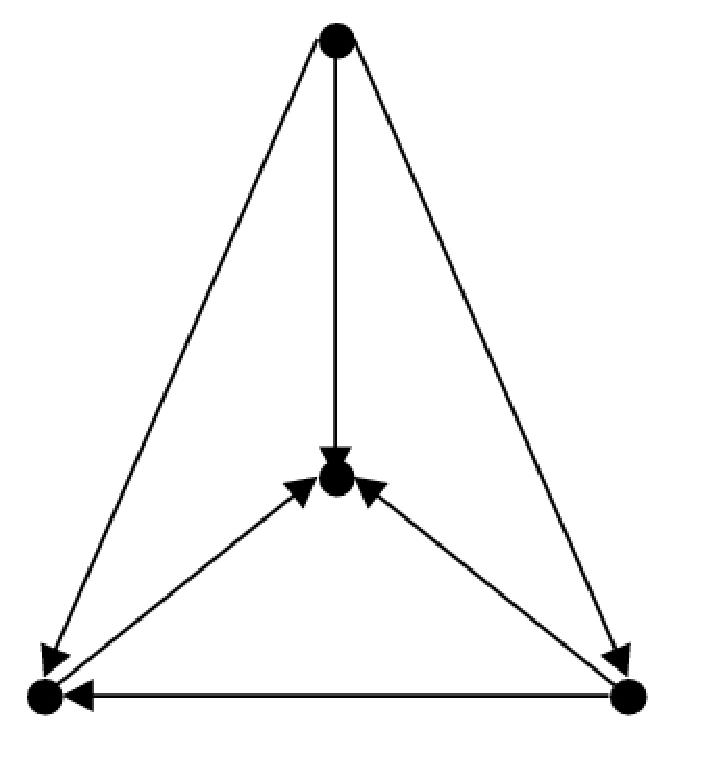
\includegraphics[scale=0.15]{figuras/capitulo2/dirigido.eps}
	\caption{Exemplo de grafo dirigido}
	\label{dirigido}
\end{figure}

Formalmente, um grafo dirigido \textit{D} é um par ordenado \textit{(V(D), E(A))}. Que consiste de um conjunto \textit{V(G)} de vértices, um conjunto \textit{A(G)}, disjunto de \textit{V(G)}, de arcos e uma função de incidência $\psi_D$ que associa a cada arco de \textit{D} um par ordenado de (não necessariamente distintas) vértices de \textit{D}. Se \textit{a} é um arco e $\psi_D$(\textit{a}) = (\textit{u,v}), então \textit{a} é dito como como a junção de \textit{u} para \textit{v}, pode-se dizer que \textit{u} domina \textit{v} \cite{Diestel:1997}.

\subsection{Árvores e Florestas}

Um grafo acíclico é aquele que não contém ciclos. Um grafo acíclico conectado é chamado de uma árvore. As árvores com seis vértices estão apresentadas na Figura \ref{arvores_seis_vertices}. De acordo com estas definições, cada componente de um grafo acíclico é uma árvore. Por esta razão, grafos acíclicos são geralmente chamados florestas \cite{Bondy:2007}.

\begin{figure}[!h]
	\centering
	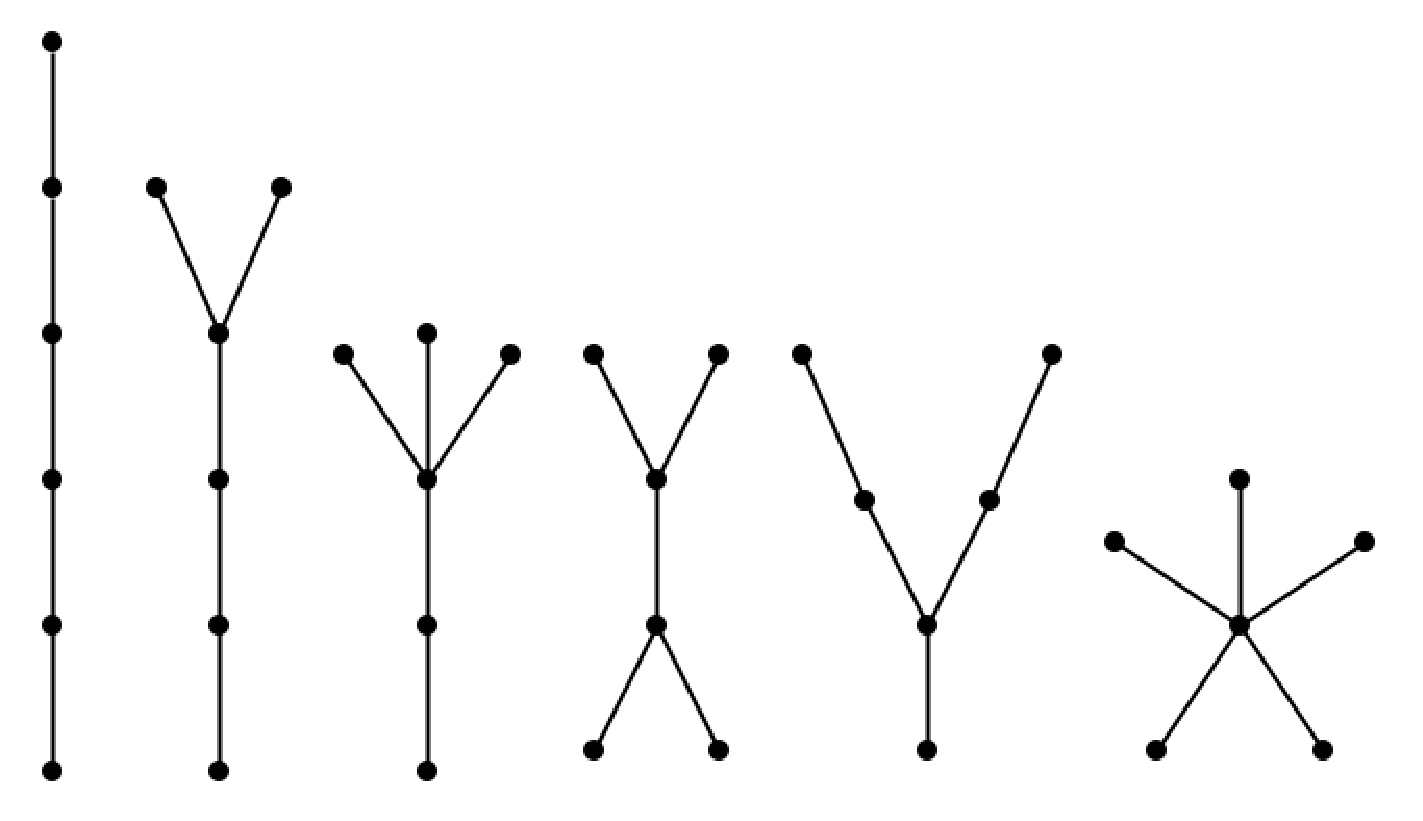
\includegraphics[scale=0.2]{figuras/capitulo2/arvores_seis_vertices.eps}
	\caption{Exemplo de árvores com seis vértices}
	\label{arvores_seis_vertices}
\end{figure}

Em uma árvore, quaisquer dois vértices são conectados por exatamente um caminho. E Diestel \cite{Diestel:1997} representa esse único caminho de ligação vértices \textit{x} e \textit{y} em uma árvore \textit{T} por \textit{xTy}.

Uma árvore com raiz \textit{T}(\textit{x}) é uma árvore \textit{T} com um vértice específico \textit{x}, chamado a raiz de \textit{T}. Em uma orientação de uma árvore com raiz, todos vértices, excluindo o vértice raiz \textit{x}, é chamado de ramificação \cite{Bondy:2007}. Um exemplo de uma árvore com raiz pode ser observado na Figura \ref{arvore_raiz}.

\begin{figure}[!h]
	\centering
	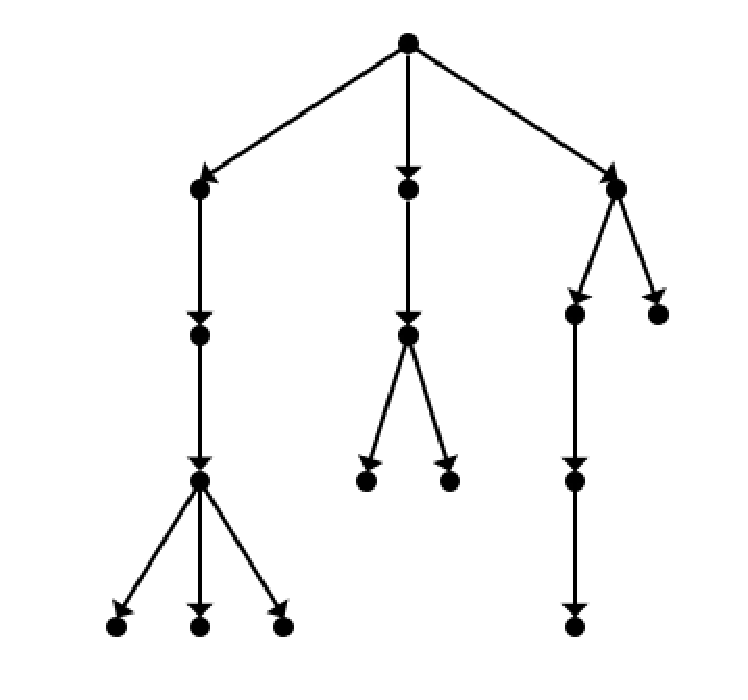
\includegraphics[scale=0.2]{figuras/capitulo2/arvore_raiz.eps}
	\caption{Exemplo de uma árvore com raiz}
	\label{arvore_raiz}
\end{figure}

\section{Algoritmos}

\subsection{Busca em Grafos}

A busca em grafos refere-se ao método de explorar o grafo, ou seja, obter um método sistemático para percorrer seus vértices e arestas. Para isto, há dois principais algoritmos, busca em profundidade (\textit{DFS - Depth First Search}) e busca em largura (\textit{BFS - Breadth First Search}). Em ambos os casos parte-se de um vértice qualquer.

\subsubsection{DFS}
A ideia por trás do \textit{DFS} é alcançar ``mais fundo'' no grafo quanto possível. A ordem em que os vértices são visitados depende da ordem em que os vizinhos de cada vértice aparecem na lista de adjacência \cite{Cormen:2001}. Considere as figuras a seguir para a exemplificação do DFS.

\begin{figure}[!h]
	\centering
	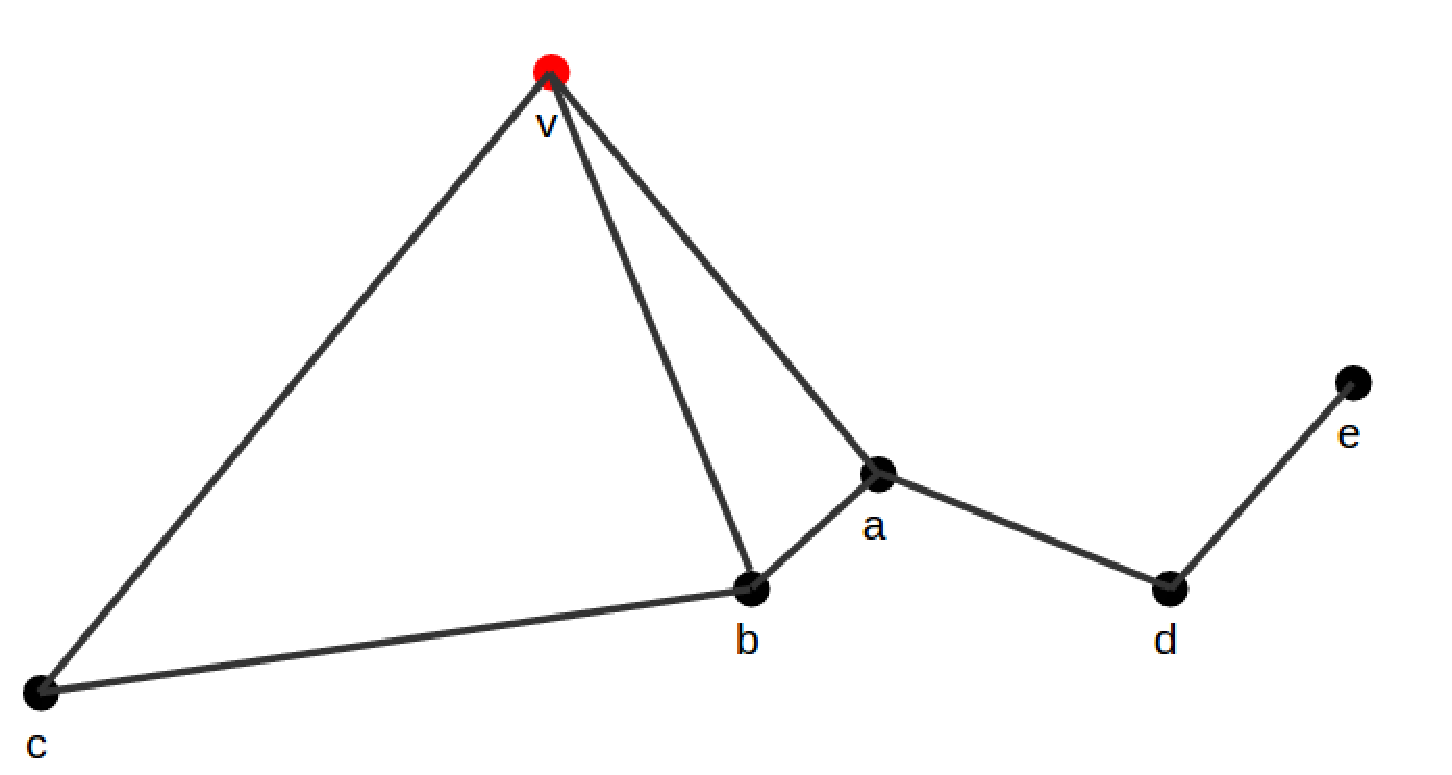
\includegraphics[scale=0.25]{figuras/capitulo2/dfs/dfs1.eps}
	\caption{Exemplo DFS etapa 1}
	\label{dfs1}
\end{figure}

A busca irá partir do vértice arbitrário \textit{v}, chamado de vértice raiz. A partir do vértice raiz é possível percorrer três arestas: (\textit{v}, \textit{a}), (\textit{v}, \textit{b}) e (\textit{v}, \textit{c}). A aresta a ser seguida será (\textit{v}, \textit{a}).

\begin{figure}[!h]
	\centering
	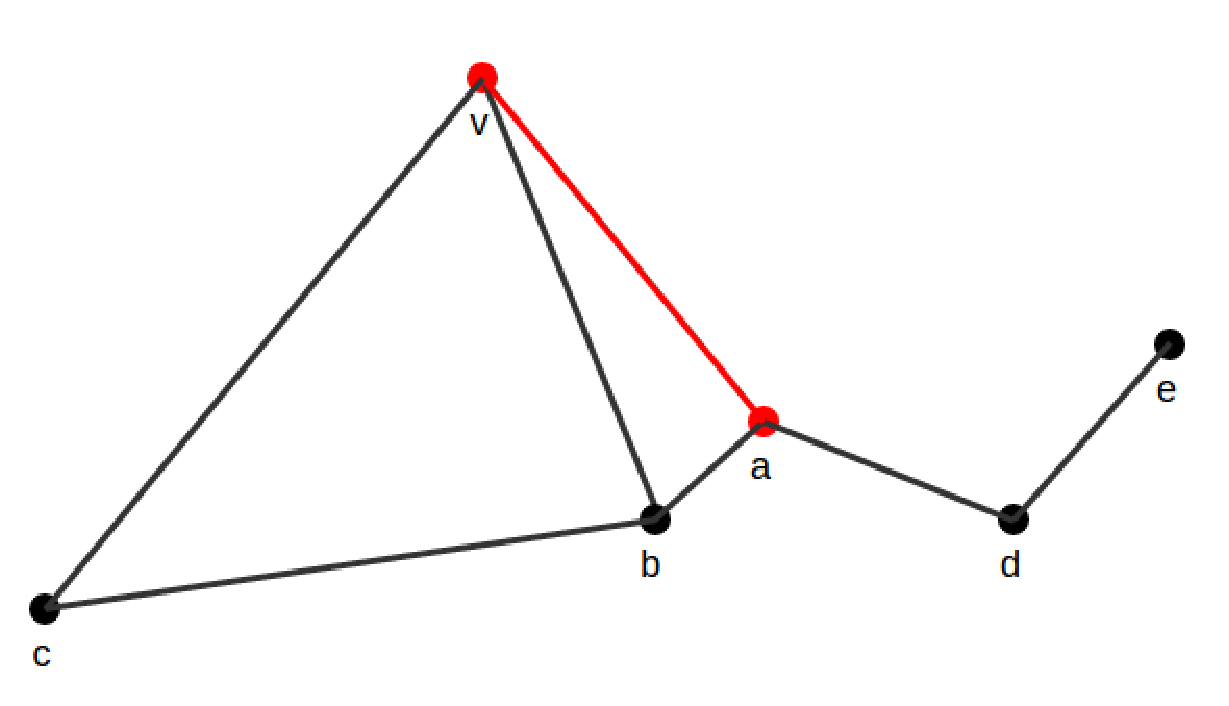
\includegraphics[scale=0.25]{figuras/capitulo2/dfs/dfs2.eps}
	\caption{Exemplo DFS etapa 2}
	\label{dfs2}
\end{figure}

O vértice \textit{a} possui três arestas, que são: (\textit{a}, \textit{v}), (\textit{a}, \textit{b}) e (\textit{a}, \textit{d}). Como o vértice \textit{v} já foi visitado, a aresta a ser seguida será (\textit{a}, \textit{b}).

\begin{figure}[!h]
	\centering
	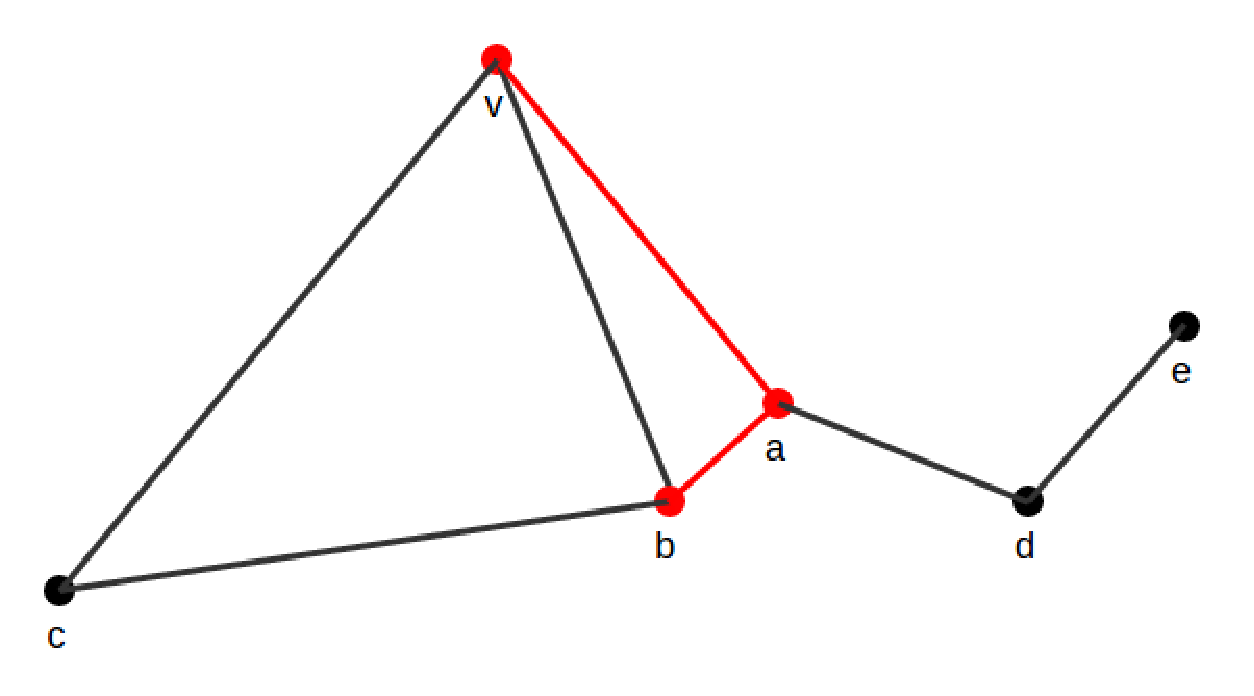
\includegraphics[scale=0.25]{figuras/capitulo2/dfs/dfs3.eps}
	\caption{Exemplo DFS etapa 3}
	\label{dfs3}
\end{figure}

A partir de \textit{b}, é possível escolher as seguintes arestas: (\textit{b}, \textit{v}), (\textit{b}, \textit{a}) e (\textit{b}, \textit{c}). Porém como os vértices \textit{v} e \textit{a} já foram visitados, a opção restante será a aresta (\textit{b}, \textit{c}).

\newpage

\begin{figure}[!h]
	\centering
	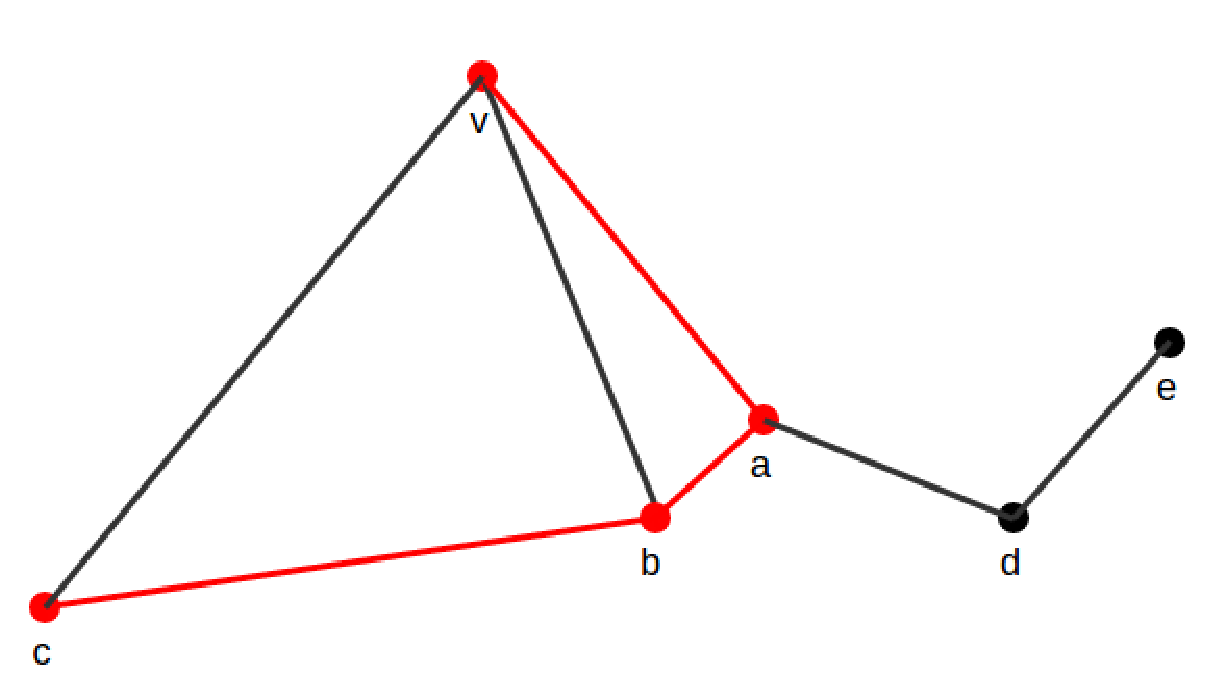
\includegraphics[scale=0.25]{figuras/capitulo2/dfs/dfs4.eps}
	\caption{Exemplo DFS etapa 4}
	\label{dfs4}
\end{figure}

Ao alcançar \textit{c}, há duas possibilidades: (\textit{c}, \textit{v}) e (\textit{c}, \textit{b}). Porém ambos os vértices \textit{v} e \textit{b} já são conhecidos. Neste caso não há para onde se aprofundar. Entretanto, ainda existem vértices não descobertos. Nesse caso, deve-se voltar até o vértice \textit{b}, verificando se há alguma aresta que leva a um vértice ainda não visitado. Caso ocorra tal situação, deve-se voltar novamente pelo caminho percorrido, chegando ao vértice \textit{a}. Em \textit{a}, a aresta (\textit{a}, \textit{d}) leva a um vértice ainda não descoberto, portanto, esse caminho deve ser tomado.

\begin{figure}[!h]
	\centering
	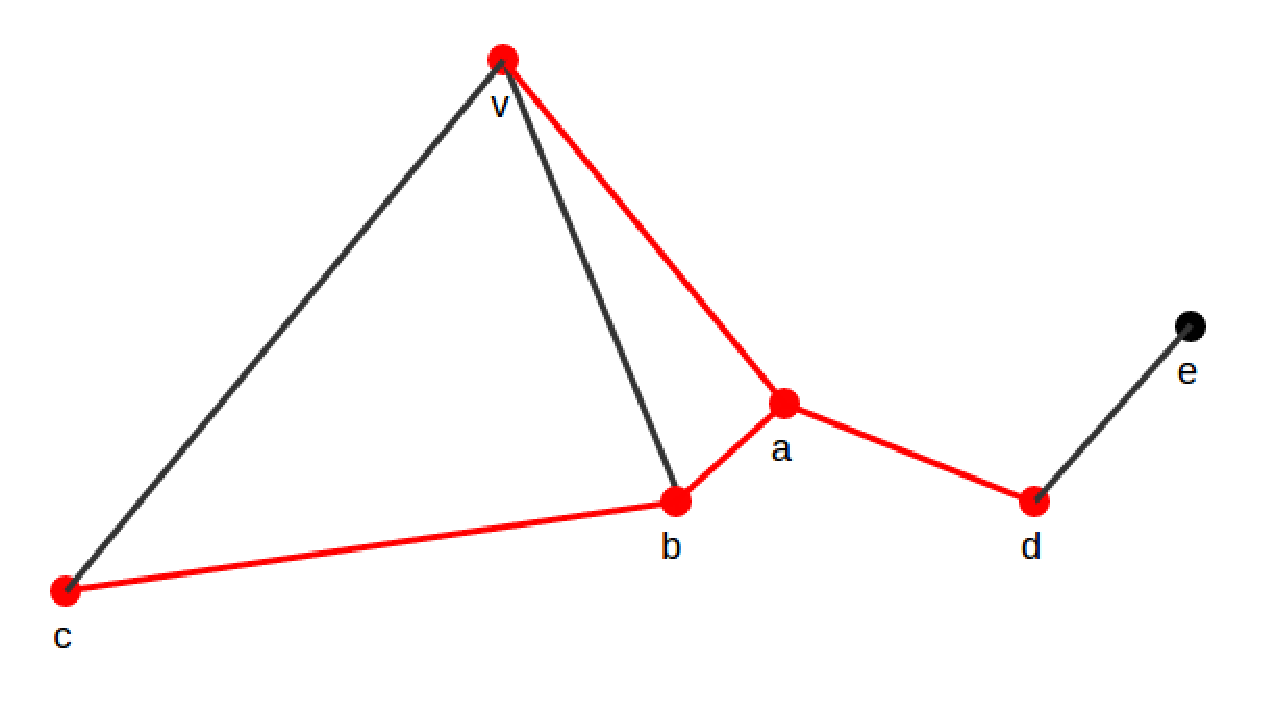
\includegraphics[scale=0.25]{figuras/capitulo2/dfs/dfs5.eps}
	\caption{Exemplo DFS etapa 5}
	\label{dfs5}
\end{figure}

Em \textit{d}, há dois caminhos a seguir: (\textit{d}, \textit{a}) e (\textit{d}, \textit{e}). Porém a única aresta que leva a um vértice não visitado é (\textit{d}, \textit{e}). Esta deverá ser seguida.

\begin{figure}[!h]
	\centering
	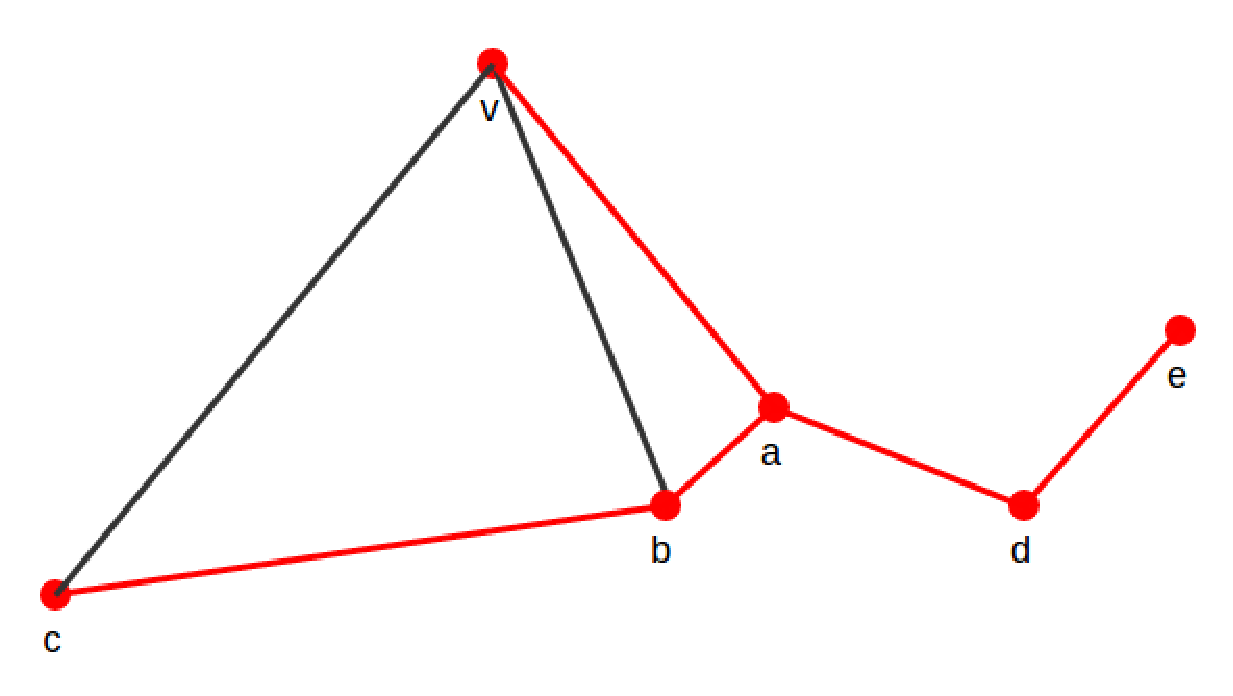
\includegraphics[scale=0.25]{figuras/capitulo2/dfs/dfs6.eps}
	\caption{Exemplo DFS etapa 6}
	\label{dfs6}
\end{figure}

Ao alcançar o vértice \textit{e}, não existem vértices não visitados, mesmo na volta no caminho. Portanto, o percurso realizado pelo \textit{DFS} pode ser observado na Figura \ref{dfs_percurso}, o qual é uma árvore.

\begin{figure}[!h]
	\centering
	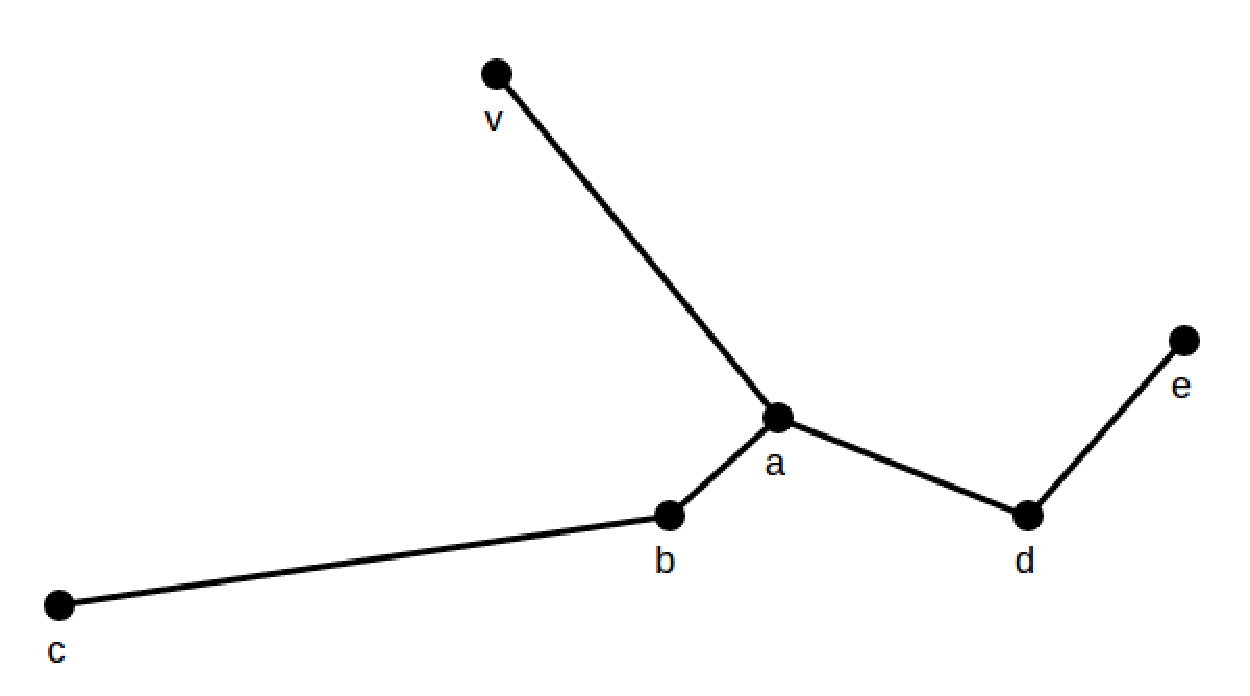
\includegraphics[scale=0.25]{figuras/capitulo2/dfs/dfs_percurso.eps}
	\caption{Percurso do DFS}
	\label{dfs_percurso}
\end{figure}

\subsubsection{BFS}

O \textit{DFS}, a partir de um vértice \textit{v}, tenta visitar algum vizinho deste, em seguida, um vizinho deste vizinho, e assim por diante. O \textit{BFS}, a partir de um vértice \textit{v}, visita todos os vizinhos de \textit{v}, quando visitado todos os vizinhos de um vértice, os vizinhos destes vizinhos serão visitados \cite{Brassard:1988}.

A Figura \ref{bfs} exemplifica o algoritmo da busca \textit{BFS}, onde as letras significam o estado da busca e a ordem de cada estado. Os vértices marcados como vermelho, representam que estes já foram visitados; os vértices marcados como azul representam que estes vértices serão os próximos a serem visitados.

\begin{figure}[!h]
	\centering
	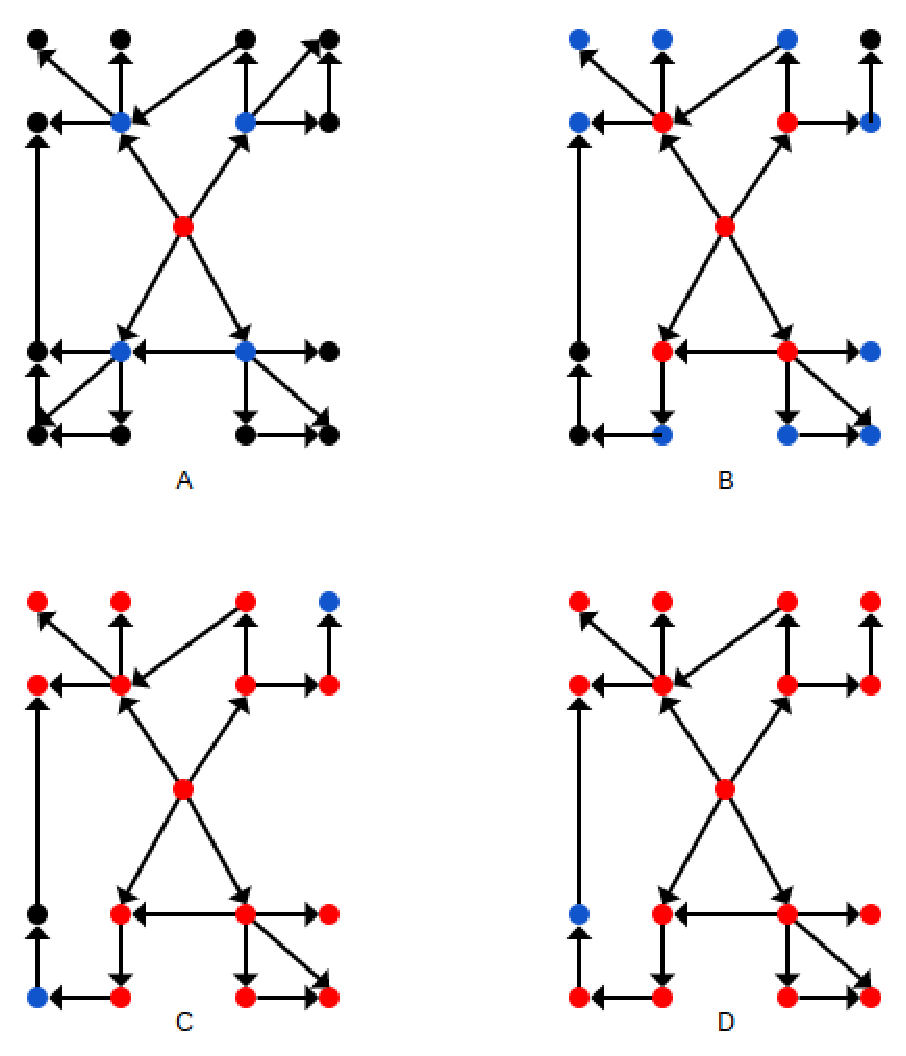
\includegraphics[scale=0.3]{figuras/capitulo2/bfs.eps}
	\caption{Percurso do BFS}
	\label{bfs}
\end{figure}

\subsection{Caminhos Mais Curtos}

Os algoritmos de menor caminho buscam obter um percurso mínimo entre dois ou mais vértices de um grafo \cite{Cormen:2001}. A seguir serão apresentados dois dos principais algoritmos de menor caminho.

\subsubsection{Algoritmo de Dijkstra}

No algoritmo de Dijkstra, escolhido um vértice como raiz da busca, este algoritmo calcula o custo mínimo deste vértice para todos os demais vértices do grafo \cite{Cormen:2001}.

O algoritmo consiste em fazer uma visita por todos os vértices do grafo, a partir de um vértice raiz, e encontrando sucessivamente o vértice mais próximo, até que todos os vértices do grafo tenham sido visitados \cite{Cormen:2001}.

\subsubsection{Algoritmo de Floyd}

Caso seja necessário saber o menor caminho entre todos os vértices do grafo, por exemplo, indicação das distâncias entre todas as cidades de um mapa, uma possível solução seria repetir o algoritmo de Dijkstra sucessivamente para todos os vértices do grafo. Porém, uma solução mais eficiente é conhecida como algoritmo de Floyd, que utiliza programação dinâmica. A ideia geral desse algoritmo é atualizar a matriz de menores distâncias \textit{n} vezes, onde \textit{n} é o número de vértices do grafo, procurando na \textit{K}-ésima interação por melhores distâncias entre pares de vértices que passem pelo vértice \textit{K} \cite{Sampaio:2005}.

\subsection{Árvore Geradora Mínima}

Uma árvore geradora de um grafo G é uma árvore contendo todos os vértices de G e as arestas que são suficientes para transformar o grafo em uma árvore. Desse modo, uma árvore geradora de custo mínimo de um grafo G é um subgrafo conexo de G, uma árvore, contendo todos os vértices de G, de modo que a soma dos pesos das arestas no subgrafo seja mínima \cite{Rezende:2002}.

Existem dois principais algoritmos para árvores geradoras mínimas \cite{Bondy:2007}:

\subsubsection{Algoritmo de Prim}

A partir de um grafo \textit{G}, não dirigido e com pesos nas arestas. Escolhe-se um vértice \textit{v} qualquer de \textit{G}, em seguida é feito um corte em \textit{G}, ({\textit{v}}, \textit{G} $\backslash$ {\textit{v}}) com respeito a \textit{v}. Inicialmente tem-se \textit{T} = {\textit{v}}, onde \textit{T} ao final será a solução do algoritmo de Prim. A aresta de menor peso, \textit{e}, desse corte é escolhida, e esta aresta é incluída em \textit{T} (\textit{T} = \textit{T} $\cup$ {\textit{e}}), até que todos os vértices tenham sido cobertos, é feito um novo corte e a aresta de menor peso é incluída em T.

\subsubsection{Algoritmo de Kruskal}

Primeiramente, ordena-se as arestas de \textit{G}. Considera-se, então, cada vértice de \textit{G} como pertencendo a uma árvore em \textit{G}, ou seja, $\textit{v}_i \in \textit{T}_i , 1 \leq i \leq |\textit{V}|$. é verificado se a menor aresta de \textit{G} une dois vértices pertencentes a árvores diferentes. Se sim, as árvores são unidas e a operação é repetida. Se não, escolhe-se a próxima aresta da lista ordenada e a operação é repetida até que todas as subárvores de \textit{G} estejam unidas.

\subsection{Programação Dinâmica}

Muitas vezes é possível dividir um problema em sub-problemas, combinando as soluções dos sub-problemas de modo a resolver a problema original. Às vezes, a maneira natural de dividir um problema sugerido pela sua estrutura pode levar a vários sub-problemas sobrepostos. Caso se tente resolver todos os sub-problemas idênticos sem se atentar a essa duplicação, é provável que o algoritmo da solução se torne exponencial. Se, por outro lado, pode-se conseguir proveito da duplicação e resolver cada sub-problema apenas uma vez, conservando a solução para utilização posterior, tem-se que o resultado do algoritmo utilizado será polinomial. A ideia subjacente de programação dinâmica é, portanto, bastante simples: evitar cálculos repetidos, geralmente mantendo uma tabela de resultados conhecidos \cite{Aho:1983}.

Existem duas principais dificuldades com a aplicação desta técnica. Em primeiro lugar, pode nem sempre ser possível combinar as soluções dos dois problemas para formar a solução de um maior. Em segundo lugar, pode haver um número inaceitável de pequenos problemas a se resolver \cite{Sedgewick:2011}.

\subsubsection{Top-Down x Bottom-Up}

A forma como a tabela na abordagem \textit{bottom-up} é preenchida não é tão intuitiva como a abordagem \textit{top-down}, pois requer algumas ``reversões'' dos sinais na recorrência. No entanto, alguns programadores sentem que a abordagem \textit{bottom-up} é mais intuitiva. A seguir é apresentada uma comparação entre as duas abordagens da programação dinâmica na tabela \ref{top-down_bottom-up} \cite{Halim:Halim:2013}:

\begin{table}[h]
	\centering
	\caption{Top-Down x Bottom-Up}
	\label{top-down_bottom-up}
	\begin{tabular}{l|l|l|}
	\cline{2-3}
	                                       & \textbf{Top-Down}                                                                                                                                                                                                              & \textbf{Bottom-Up}                                                                                                                                                                                                               \\ \hline
	\multicolumn{1}{|l|}{\textbf{Prós}}    & \begin{tabular}[c]{@{}l@{}}1. É uma transformação natural da\\ busca completa recursiva.\\ \\ \\ 2. Computa os sub-problemas somente\\ quando necessário (às vezes isso é mais\\ rápido).\end{tabular}                         & \begin{tabular}[c]{@{}l@{}}1. Mais rápido se muitos sub-problemas\\ são revisitados, pois não há sobrecarga\\ de chamadas recursivas.\\ \\ 2.Pode economizar espaço de memória\\ com a técnica \textit{on-the-fly}.\end{tabular} \\ \hline
	\multicolumn{1}{|l|}{\textbf{Contras}} & \begin{tabular}[c]{@{}l@{}}1. Mais lento se muitos sub-problemas\\ são revisitados, devido à sobrecarga de\\ chamadas recursivas.\\ \\ 2. Se existem M estados, tamanho da\\ tabela pode ser de até $\theta$(M ).\end{tabular} & \begin{tabular}[c]{@{}l@{}}1. Para programadores familiarizados\\ com recursão, pode não ser intuitivo.\\ \\ 2. Se existem M estados, todos serão\\ serão visitados e os valores serão\\ preenchidos.\end{tabular}               \\ \hline
	\end{tabular}
\end{table}

\section{Reutilização de Software}

A reutilização de software tem como objetivos aumentar a qualidade e produtividade no desenvolvimento, pois busca evitar duplicidade de código e do esforço aplicado para desenvolver determinadas tarefas, reaproveitando o máximo possível experiências passadas \cite{Lucredio:2009}.

Todas as formas de reutilização de software usam algum tipo de abstração.  Essa é uma característica importante presente nas técnicas de reutilização, pois facilita aos desenvolvedores o uso. Sem abstrações, os desenvolvedores deveriam analisar todos os artefatos reutilizáveis buscando entender como cada um funciona e como e quando devem ser utilizados \cite{Krueger:1992}.

Os próximos subtópicos irão apresentar temas deste trabalho que estão diretamente relacionados à reutilização de software.

\subsection{Frameworks}

Frameworks compartilham técnicas de reutilização em geral e são considerados uma importante parte da cultura de desenvolvimento no mundo da orientação a objetos \cite{Johnson:1997}.

Fayad e Schimidt, em seu artigo \cite{Fayad:Schimidt:1997} sobre frameworks de aplicações orientadas a objetos, mostram quais são os principais benefícios no uso de frameworks, dentre eles: modularização, reutilização, extensibilidade e inversão de controle.

\begin{itemize}
	\item \textbf{Modularização:} Frameworks encapsulam e interfaceiam alguns detalhes de implementação. Isso reduz o esforço necessário para entender e manter partes do software existente, pois basta ao desenvolvedor usar o que lhe é oferecido sem necessariamente entender qual a implementação do framework.

	\item \textbf{Reutilização:} As interfaces providas por frameworks ajudam também na reutilização através da definição de componentes genéricos, que podem ser aplicadas em outras aplicações. Assim sendo, soluções comuns para sistemas diferentes podem ser usadas da mesma forma sem a necessidade de recriação das mesmas. Entende-se então, que estas soluções são pensadas uma única vez, e ao estarem presentes em um framework, basta que sejam usadas.

	\item \textbf{Extensibilidade:} Este é um dos principais pontos positivos dos frameworks, pois estes fornecem métodos e interfaces estáveis que outras aplicações irão utilizar. Essas aplicações devem poder usar esses métodos, visando resolver problemas parecidos em diferentes contextos. Uma boa estrutura de extensibilidade é essencial para garantir a customização de novos serviços e funcionalidades das aplicações.

	\item \textbf{Inversão de controle:} A inversão de controle ocorre devido a forma como serão processados e entendidos muitos dos eventos de uma aplicação, que ficam invisíveis ao desenvolvedor quando este usa um framework, pois é o próprio framework quem decide o conjunto de métodos que será invocado para realizar uma determinada tarefa da aplicação.
\end{itemize}

\subsubsection{Frameworks e Reutilização de Software}

A tecnologia de reutilização ideal provê componentes que podem facilmente ser conectados para criar um novo sistema. Não é necessário ao desenvolvedor ter conhecimento de como o componente é implementado, e geralmente é fácil para ele aprender como o utilizar. O resultado é que o sistema será eficiente, fácil de manter e confiável \cite{Johnson:1997}.

Frameworks são aplicações especializadas em prover classes e componentes abstratos que podem ser usados por outros sistemas. Estes proveem técnicas de reutilização robustas e de maior granularidade. Sendo aplicações independentes é mais fácil usá-los em um maior número de sistemas \cite{Johnson:Foote:1988}.

Para se alcançar a aplicação efetiva de um dado framework é, necessário ao desenvolvedor conhecer as interfaces que o framework proporciona antes de poder usá-las. Como podem existir diversas interfaces complexas, aprender a usar um novo framework pode ser difícil. Porém, os frameworks são poderosos e o tempo gasto em sua aprendizagem é recompensado, pois podem reduzir a quantidade de esforço aplicado para se desenvolver uma nova aplicação que os usem \cite{Johnson:1997}.

Ao longo do tempo, tornou-se muito caro desenvolver aplicações complexas a partir do zero. Isso porque todos os componentes que são desenvolvidos devem passar por um criterioso processo de validação e manutenção, e isso ocorre sempre que um novo sistema é desenvolvido. Ao se usar frameworks, pode-se desenvolver componentes comuns e os processos citados são feitos em um único local \cite{Fayad:Schimidt:1997}.

% Falar sobre os cinzas.
As técnicas de reutilização são diferentes de acordo como o tipo do framework utilizado, esses tipos podem ser ``\textit{white box}'' ou ``\textit{black box}''. O primeiro diz respeito a quando o código do framework é aberto e visível ao desenvolvedor, dessa forma, este pode estudar a implementação do framework e modificar o código de determinadas partes de acordo com suas necessidades. Os frameworks do tipo ``\textit{black box}'' disponibilizam apenas interfaces ao desenvolvedor para que este possa usá-las, a forma como tudo é implementado e processado é desconhecida. No primeiro tipo, têm-se uma maior flexibilidade, porém, o uso é mais complexo ao desenvolvedor. No segundo, o uso é bem simples, porém, não existe flexibilidade para mudança da implementação \cite{Kroth:2000}.

Além dos tipos de frameworks, estes também podem ser divididos quanto a sua aplicabilidade. Podem ser desenvolvidos para serem aplicados em qualquer domínio, de forma genérica sem se preocupar com algo específico \textit{frameworks horizontais}, ou podem ser desenvolvidos visando atender um tipo específico de domínio de problemas, \textit{frameworks verticais}. Essas características dependem das necessidades apresentadas ao se trabalhar com frameworks, e isso impacta como será aplicada a reutilização \cite{Kroth:2000}.

Na Engenharia de Software, busca-se cada vez mais o aumento da produtividade e da qualidade dos sistemas desenvolvidos. A reutilização de software, ao contrário de todas as outras partes de um sistema, é um fator que pode acarretar o aumento desses fatores, considerando que ao se utilizar componentes já desenvolvidos e depurados pode-se reduzir o tempo de desenvolvimento, de testes e as chances de ocorrência de erros que poderiam advir se fosse necessário a criação destes novos artefatos \cite{Silva:2000}.

Além de ganhos na produtividade e na qualidade a reutilização advinda dos frameworks podem trazer ganhos de desempenho, confiabilidade e interoperabilidade de software \cite{Fayad:Schimidt:1997}.

\subsubsection{Frameworks e Padrões}

Padrões representam soluções recorrentes para problemas no desenvolvimento de software em um contexto específico. Tanto os padrões como os frameworks são técnicas de reutilização, a grande diferença é que os frameworks 	se concentram na reutilização de estruturas, algoritmos e implementações em uma dada linguagem de programação. Já os padrões focam em apresentar desenhos abstratos de como resolver problemas; como microarquiteturas de software \cite{Fayad:Schimidt:1997}.

Um padrão descreve um problema a ser resolvido e apresenta uma solução e o contexto em que essa solução funciona, nomeia uma técnica e descreve seus custos e benefícios \cite{Johnson:1997}.

Quando um framework é implementado diversas, vezes este também pode ser considerado um padrão \cite{Johnson:1997}. O MVC (\textit{Model / View / Controller}) é um framework conceitual de interface com usuário que é considerado um padrão \cite{Almeida:2006}.

Quando usados em conjunto com padrões, os frameworks podem aumentar significativamente a qualidade do software e reduzir o esforço de desenvolvimento \cite{Fayad:Schimidt:1997}.

\subsection{Padrões de Projeto}

Os padrões de Projeto são parte da vanguarda da tecnologia orientada a objetos e este tema tem estado em constante crescimento no decorrer dos tempos. A proposição por trás dos padrões é que a qualidade do software pode ser medida objetivamente, isso considera que ao se analisar o design de um padrão este pode ser considerado bom ou ruim, e assim resultando em uma boa ou má qualidade \cite{Shalloway:Trott:2004}.

Alexander, em seu livro \cite{Alexander:1979} sobre padrões de construção, diz:

\begin{quote}
	``cada padrão descreve um problema no nosso
ambiente e o cerne da sua solução, de tal forma que você possa usar essa solução mais
de um milhão de vezes, sem nunca fazê-lo da mesma maneira''
\end{quote}

No livro de padrões de projeto \cite{Gamma:Helm:Johnson:Vlissides:1995}, o autor concorda com as afirmações de Alexander. A diferença principal é que no âmbito de software os padrões são expressos em termos de objetos e interfaces ao invés de paredes e portas. Porém, ambos os tipos os padrões dizem respeito a uma solução para um problema em um contexto geral. Além disso, Gamma considera que um padrão é dividido em quatro partes principais, que são:

\begin{itemize}
	\item \textbf{Nome:} Usado para descrever um problema de projeto, suas soluções e consequências em uma ou duas palavras. Quando um padrão possui um nome fica mais fácil de definir um vocabulário comum para tratar deste com outras pessoas.
	\item \textbf{Problema:} O problema está ligado diretamente a situação em que deve ser aplicado o padrão, ou seja, qual o contexto. Algumas vezes o problema pode conter uma lista de condições que devem ser satisfeitas para que se possa alcançar sentido na aplicação do padrão.
	\item \textbf{Solução:} Esta descreve todos os elementos que compõem o padrão, seus relacionamentos, responsabilidades e colaborações. É fornecida uma descrição abstrata de um problema de projeto e o arranjo geral de classes e objetos que resolvam o padrão. Não há uma solução ou implementação concreta, pois padrões são desenhados para serem usados em muitas situações diferentes.
	\item \textbf{Consequências:} As consequências apresentam uma série de resultados concernentes da aplicação do padrão, devem ser apresentadas vantagens e desvantagens. São elementos críticos que entram na decisão da aplicação ou não do padrão que está em questão.
\end{itemize}

\subsubsection{Por que usar Padrões de Projeto?}

Os dois pontos que melhor justificam o uso de padrões de projeto são brevemente descritos a seguir de acordo com \cite{Shalloway:Trott:2004}:

\begin{itemize}
	\item \textbf{Soluções Reutilizáveis:} O tempo gasto para aprender a utilizar determinado padrão vale a pena pela reutilização que é oferecida. Têm-se o benefício de aplicar o que foi aprendido para diversos projetos. Depois de ter o conhecimento fixado, não é necessário reinventar soluções para problemas recorrentes, basta reutilizar o que os padrões oferecem.
	\item \textbf{Terminologia Comum:} Quando se está em um grupo de trabalho é necessário uma base de vocabulário e pontos de visão do problema comuns. Os padrões de projeto providenciam um ponto comum de referência durante as fases de análise e \textit{design} de um projeto.
	\item \textbf{Perspectiva de alto nível do problema:} Os padrões dão aos desenvolvedores essa perspectiva e ajudam na análise e entendimento dos problemas, facilitando a elaboração de uma melhor solução.
\end{itemize}

Gamma ainda diz que os padrões podem ajudar na refatoração de projetos. Um das grandes dificuldades no desenvolvimento de software é que este tem de ser frequentemente reorganizado ou refatorado, os padrões de projeto ao oferecerem soluções comuns e já consolidadas podem reduzir a quantidade de refatoração que deverá ser feita mais tarde \cite{Gamma:Helm:Johnson:Vlissides:1995}.

\subsubsection{Classificação de Padrões de Projeto}

Em \cite{Gamma:Helm:Johnson:Vlissides:1995}, foram definidos e classificados 23 padrões. Essa classificação está feita de acordo com dois critérios: \textbf{finalidade} e \textbf{escopo}. O primeiro critério diz respeito ao que o padrão faz, a finalidade pode ser de criação, estrutural ou comportamental. Os padrões com finalidade de criação se preocupam com o processo de criação de objetos. Os estruturais focam em composições de classes ou objetos. Os comportamentais caracterizam as maneiras que as classes ou objetos interagem e distribuem responsabilidades.

O segundo critério especifica se o padrão é de classe ou objeto. Os padrões de classes lidam com relacionamentos entre classes e suas subclasses, para isso são utilizados relacionamentos de herança. E os padrões de objetos são mais dinâmicos, pois lidam com relacionamentos entre objetos que podem ser mudados em tempo de execução.

A seguir, têm-se uma breve descrição do padrão ``\textit{Abstract Factory}'', como foi definido em \cite{Gamma:Helm:Johnson:Vlissides:1995}.

\subsubsection{Abstract Factory}

Esse padrão fornece uma estrutura para criação de famílias de objetos relacionados sem a necessidade de definir suas classes concretas. A figura \ref{abstract factory} apresenta o modelo do ``\textit{Abstract Factory}''.

\newpage

\begin{figure}[!h]
	\centering
	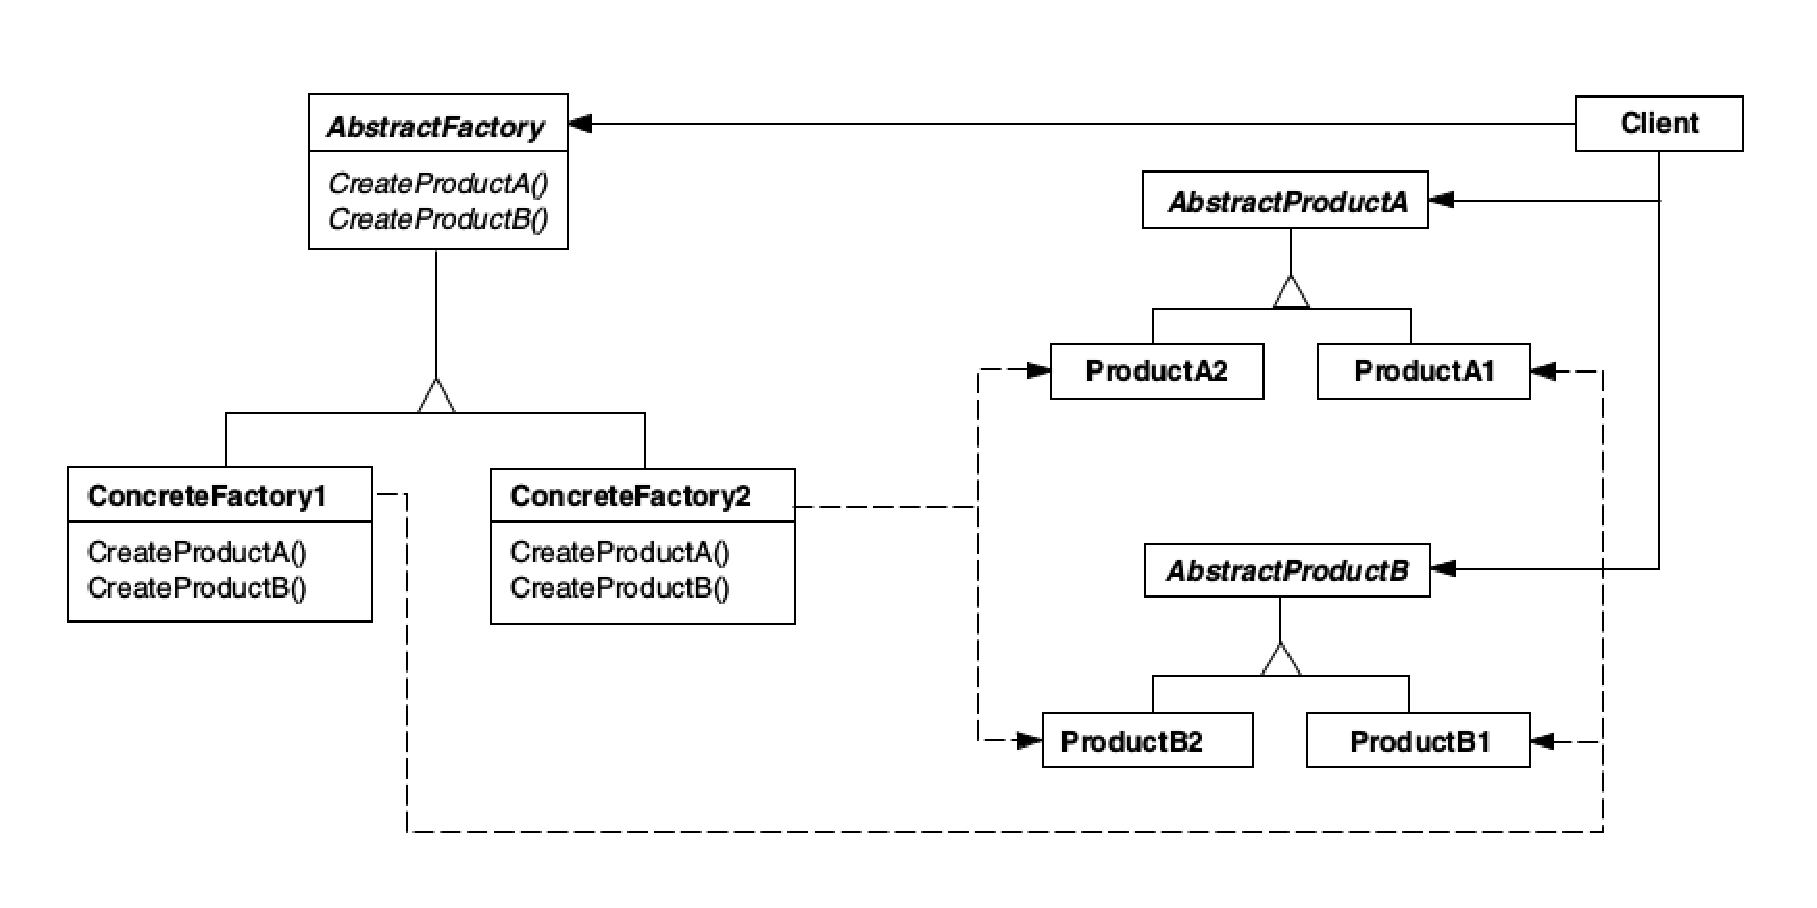
\includegraphics[scale=0.5]{figuras/capitulo2/abstract_factory.eps}
	\caption{Modelo genérico do Abstract Factory}
	\label{abstract factory}
\end{figure}

O modelo da figura apresenta cinco tipos de classes. ``\textit{Abstract Factory}'', ``\textit{Concrete Factory}'', ``\textit{Abstract Product}'', ``\textit{Product}'' e ``\textit{Client}''.

\begin{itemize}
	\item \textbf{\textit{Abstract Factory:}} Faz declarações de interfaces para criação de quaisquer produtos;
	\item \textbf{\textit{Concrete Factory:}} Essas classes já estão focadas no tipo de produtos que vão criar e implementam os métodos abstratos para essa criação;
	\item \textbf{\textit{Abstract Product:}} Classes abstratas que declaram interfaces para um determinado tipo de produto que deverá ser criado;
	\item \textbf{\textit{Product:}} Classes que representam o próprio produto que deverá ser criado, são as classes que são chamadas pelos métodos de criação presentes nas ``\textit{Concrete Factory}'';
	\item \textbf{\textit{Client:}} É a classe que representa quem irá fazer as chamadas aos métodos de criação. Não é necessário que conheça de fato as classes concretas de produto, pois apenas faz uso das interfaces declaradas em ``\textit{Abstract Factory}'' e ``\textit{Abstract Product}''; a primeira para criar os produtos, e a segunda para usá-los.
\end{itemize}

Este padrão oferece algumas vantagens e desvantagens que são apresentadas a seguir:

\begin{itemize}
	\item \textbf{Isolamento de classes concretas:} O cliente pode trabalhar com as criações dos produtos sem necessariamente conhecer as classes concretas que existem por traz, pois este trabalha apenas com as interfaces abstratas providas.
	\item \textbf{Fácil troca de famílias de produtos:} Basta trocar qual é a classe concreta que deverá ser usada que todo o comportamento dos produtos irá se alterar de acordo com essa classe. Isso pode ser feito facilmente no momento de instanciação da fábrica.
	\item \textbf{Harmonia entre produtos:} Como o padrão permite aos clientes trabalharem apenas com uma família por vez, fica fácil alcançar harmonia, pois todos os produtos da família estão de alguma forma relacionados.
	\item \textbf{Suporte a novos tipos de produtos é difícil:} Como a interface do ``\textit{Abstract Factory}'', no início, cria uma quantidade fixa de produtos para serem implementados, alterar isso fica difícil, pois é necessário mexer na classe principal e criar as subclasses concernentes.
\end{itemize}

% A milene pediu pra cadenciar, pq o tópico caiu de paraquedas

\subsection{Serviços}

De uma maneira geral, serviços são atividades providas e realizadas por uma máquina ou um humano. No desenvolvimento de software, serviços são considerados um bloco de construção reutilizável que oferece uma funcionalidade particular. A noção de reusabilidade apresentada lembra a reutilização antes comentada no conceito de componentes. De fato, essas duas abordagens estão próximas, pois representam uma ideia de desenvolvimento comum, onde blocos de software são construídos para serem usados por atores diferentes e em outros locais \cite{Stojanovic:Dahanayake:2005}.

Com o advento dos serviços, surgiu um novo termo, a ``Orientação a serviços''. Que ocorre quando alguns processos são modelados e construídos como unidades bem definidas e formam serviços. Que são encapsulados em componentes de software para serem usados por outras aplicações dando a ideia de um sistema provedor (o sistema que provê o serviço) e um sistema consumidor (que consome os serviços prestados) \cite{Victorino:Brascher:2009}.

Se todas as aplicações usassem a mesma interface de programação e o mesmo protocolo de interoperabilidade, todo o trabalho de software seria mais simples. Essa é a premissa que trouxe o desenvolvimento orientado a serviços para o mundo da tecnologia da informação. quando se desenvolve dessa forma, os serviços tornam-se a base para a criação de novas estratégias de solução \cite{Newcomer:Lomow:2004}.

Apesar das abordagens de orientação a serviços e orientação a componentes serem bem similares, no livro \cite{Stojanovic:Dahanayake:2005}, são apresentadas algumas diferenças entre as mesmas, que são:

\begin{itemize}
	\item O tempo de integração. Na orientação baseada em componentes a integração com a aplicação desenvolvida ocorre no momento da construção; enquanto na orientação a serviços a integração pode ocorrer antes ou durante a execução, pois apenas as descrições dos serviços estão disponíveis no momento da execução.
	\item Nos serviços o foco é a descoberta, existindo uma ênfase mais forte na separação entre a descrição do serviço e a implementação. Nos componentes é a composição, onde as partes são integradas diretamente na aplicação.
	\item Serviços são mais voltados para tarefas dinâmicas, ao contrário dos componentes que são mais voltados para pontos estáticos. Porém, esse comportamento pode ser feito também em componentes.
	\item A orientação a componentes dá mais responsabilidade para o ambiente e execução da própria aplicação. Os serviços não são necessariamente dessa forma, pois podem estar presentes em outras máquinas e servidores externos.
\end{itemize}

% também caiu de paraquedas
\subsubsection{Web Services}

Os serviços são informatizados por tecnologias interoperáveis, que são capazes de se comunicar entre si, e isso independe da plataforma e linguagem de programação utilizadas. Dentre essas tecnologias, os ``\textit{Web Services}'' (serviços web) se destacam. Esses serviços fornecem um modo padronizado de integrar aplicativos web, e assim, organizações podem se comunicar sem que uma tenha conhecimento abrangente dos sistemas da outra \cite{Victorino:Brascher:2009}.

Um ``\textit{Web Service}'' é uma noção abstrata que deve ser implementada por um agente concreto, este agente é um pedaço de software que envia e recebe mensagens. O serviço é o recurso caracterizado pela funcionalidade abstrata que é servida.

O XML hoje é amplamente utilizado quase como o protocolo HTTP e faz parte da solução para aplicação de ``\textit{Web Services}''. Normalmente, usado para realizar a formatação dos dados \cite{Alonso:Casati:Kuno:Machiraju:2010}.

Simplificando, os ``\textit{Web Services}'' possuem três características e tecnologias principais que são usadas para desenvolvê-los: o XML, que é a especificação sobre a qual estes são construídos; o WSDL, que provê as interfaces fundamentais que serão usadas, e SOAP, que é responsável pela comunicação com outros serviços. Pode-se dizer que um ``\textit{Web Service}'' deve fornecer interfaces de uso simples e se comunicar facilmente com outros serviços \cite{Newcomer:Lomow:2004}.

\subsubsection{Serviços RESTFul}

REST é um estilo arquitetural para sistemas hipermídia distribuídos, reunindo um grupo de critérios que serão incorporados ao projeto de aplicações distribuídas. Os Serviços RESTful são serviços web que seguem os critérios REST \cite{Filho:2009}.

O uso de serviços RESTFul ganhou um grande impulso no desenvolvimento de aplicações distribuídas baseadas em padrões WEB tradicionais. Esses serviços são leves, práticos e fáceis de serem integrados em várias aplicações \cite{Rosenberg:Curbera:Duftler:Khalaf:2008}.

Os serviços da web estão a cada dia buscando soluções mais simples e mais leves para compor suas funcionalidades. Os serviços RESTFul introduzem um novo tipo de abstração que busca oferecer as funcionalidades já existentes dos serviços da \textit{web} comuns. Porém, de uma forma mais leve e simples \cite{Pautasso:2009}.

De acordo com \cite{Filho:2009}, os serviços RESTFul possuem cinco conceitos importantes, que são descritos a seguir:

\begin{itemize}
	\item \textbf{Recurso:} É uma abstração ou conceito relevante para o domínio tratado. Os recursos podem ser concretos ou abstratos e têm-se grande flexibilidade para definição dos mesmos. Um serviço pode ter mais de um recurso sem afetar a sua qualidade.
	\item \textbf{Representação:} É a representação de um recurso, apresentando informações sobre o mesmo. Dependendo do serviço e do nível de abstração, são mostradas mais ou menos informações dos recursos. A representação é uma serialização do recurso em uma linguagem específica, as mais usadas são: XML, XHTML e JSON. Um serviço pode mostrar mais de um tipo de serialização de seus recursos, basta que as requisições informem qual o formato desejado que o serviço irá apresentar os dados na serialização correta.
	\item \textbf{Identificador Uniforme:} Cada recurso deve ter ao menos um identificador para localização do mesmo. Se não existe um identificador uniforme, não se pode considerar que um objeto é um recurso. Pode-se ter ilimitados identificadores para um mesmo recurso.
	\item \textbf{Interface Unificada:} A interface unificada diz respeito a todos os serviços utilizarem o mesmo protocolo, no caso, o HTTP. Dessa forma, um cliente que conheça esse protocolo pode facilmente se utilizar dos métodos que são proporcionados por ele para fazer requisições nos serviços disponíveis.
	\item \textbf{Escopo de Execução:} Neste caso, o serviço RESTFul também se utiliza do protocolo HTTP, porém, diz respeito aos parâmetros que devem ser enviados junto da requisição para que o serviço possa tratar o recurso corretamente. Pode ser, por exemplo, a identificação de um objeto em um conjunto de recursos.
\end{itemize}

% Considerações Finais